\documentclass[10pt,a4paper]{article}
\usepackage[utf8]{inputenc}
\usepackage{amsmath}
\usepackage{amsfonts}
\usepackage{amssymb}
\usepackage{a4wide} %Wider margins
\usepackage[english]{babel} %English dictionary for hyphenation and definitions, e.g. Table vs. Tabel
\usepackage[official]{eurosym} %Support for Euro-sign
\usepackage[utf8]{inputenc} %Support for internationalization, e.g. é vs.\’e
\usepackage{amsmath,amssymb,amsthm} %Support for mathematical formulas and symbols
\usepackage{fancyhdr} %Fancy headers
\usepackage{hyperref} %Creates clickable links
\usepackage{graphicx} %Support for grahpics
\usepackage{nopageno} %Support for removal of pagenumbers
\usepackage{tabularx}
\usepackage{enumitem}
\usepackage{xspace}
\usepackage{array}
\usepackage{algorithm,algpseudocode}
\usepackage{float}
\usepackage{mathtools}
\usepackage[table, xcdraw,dvipsnames]{xcolor}
\usepackage[titletoc,toc,title]{appendix}
\usepackage{listings}
\usepackage{pdfpages}
\usepackage{footmisc}
\usepackage{attachfile2}
\usepackage{subfig}
\usepackage{amsmath}
\usepackage{rotating}
\usepackage{algorithm}
\usepackage{multirow}
\usepackage{algpseudocode}
\usepackage{rotating}

\graphicspath{ {./ThesisFigures/} }

\hypersetup{
    pdftitle={}, %PDF-file will be given a proper title when viewed in a reader
    hidelinks %PDF-file will be given clickable, yet not visible links when viewed in a reader
}
\newcommand{\documenttitle}{Dataset exploration}
\newcommand{\documentsubtitle}{A case study for a computational biology framework}


\newcommand{\true}{{\sc True}\xspace}
\begin{document}
	
	\begin{titlepage}
		
		\center
		
		\vspace*{3cm}
		
		\textbf{\huge \documenttitle}
		
		\textit{\LARGE \documentsubtitle}
		
		\vspace*{2cm}
		
		\large
		\centering
		T.P.A.~\textsc{Beishuizen}~(0791613)\\
		Biomedical Engineering - Computational Biology\\
		Computer Science - Data Mining\\
		Eindhoven, University of Technology\\
		Email: \texttt{t.p.a.beishuizen@student.tue.nl}
		
		\vfill
		
		\vspace*{1cm}
		
		\today
		
	\end{titlepage}
	
	\tableofcontents
	
	%\newpage
	
	\pagestyle{fancy}
	%Abbreviations used by fancyhdr:
	%E Even page
	%O Odd page
	%L Left field
	%C Center field
	%R Right field
	%H Header
	%F Footer
	\fancyhead{} % clear all header fields
	\fancyfoot{} % clear all footer fields
	\renewcommand{\headrulewidth}{0.4pt}
	\renewcommand{\footrulewidth}{0.4pt}
	
	\fancyhead[L]{\rightmark}
	\fancyfoot[C]{\thepage}
	\fancyhead[R]{T.P.A. Beishuizen}
	
	
	\clearpage
	
	\section{Introduction}
	\label{sec:Introduction}
	
	% Quick explanation for biomedical data
	Many biomedical datasets have been created to use for expansion of biomedical knowledge and improvement of healthcare. Biomedical data is a generalizing term that describes multiple data types\cite{gehlenborg2010visualization}. Examples of biomedical data are micro-array data\cite{brazma2001minimum}, mass spectrometry data\cite{cottrell1999probability, dettmer2007mass} and nuclear magnetic resonance data\cite{capitani2017nuclear}, but also clinically derived data\cite{liu2012data, sittig2008grand} and survey data\cite{magni1990chronic}. From a bio-informatics perspective these biomedical data types vary significantly\cite{gehlenborg2010visualization} and therefore extracting information out of biomedical data is not a trivial task. A framework for biomedical data analysis can help guiding biomedical engineers in their process of information extraction from their biomedical datasets. The framework can provide different options in processing the data, taking into account common dataset issues\cite{bertolazzi2008logic, piatetsky2003microarray,lommen2009metalign} and approaches to reach a certain goal\cite{holzinger2014knowledge, wilkins2009proteomics}. Currently available frameworks however mainly focus on the integration of databases\cite{teodoro2009biomedical, doi:10.1093/nar/gkm1037}, are made specifically for one research area\cite{sturn2002genesis, karnovsky2011metscape, tabas2012genecodis3} or are limited to one specific type of analysis\cite{faul2007g}. A framework that combines database integration, multiple research areas and multiple types of data analysis would be very beneficial for biomedical engineers, guiding them through their biomedical data analysis projects.
	
	% Analysis techniques
	Before actual analysis can be done, a course of action needs to be chosen and the dataset usually needs to be preprocessed. This preprocessing can vary from removing redundant values to normalizing data. The course of action can vary from a type of quality testing to starting with a certain analysis technique. To find the right types of preprocessing and data analyses, initial analysis can be done. The goal of this research is \textit{to find initial analyses that help finding suitable preprocessing algorithms and show a direction for data analysis}.
	
	% Meta-features
	A possible way of finding out possible suitable preprocessing techniques is by using meta-features. Meta-features are dataset specific values that have information on a certain aspect of the dataset\cite{kluegl2009meta} (Appendix \ref{app:MetaFeatures}). With the use of the information available in these meta-features suitable preprocessing and analysis techniques can be found and help the scientist in its research.
	
	\section{Background}
	\label{sec:Background}
	
	% Introduction
	First two datasets are introduced. These datasets are different in multiple ways and several preprocessing and analysis techniques are known to be suitable for these datasets. Secondly, multiple well known preprocessing and analysis techniques are discussed that are used often in the initial phases of research.
	
	\subsection{Datasets}
	\label{subsec:Datasets}
	
	% Introduction
	Two different datasets are used to show the use of the datasets. Each of the datasets has different aspects, which makes them useful for testing a wider variety of meta-features. These datasets are based on micro organisms and hepatitis:
	
	\begin{itemize}
		\item % MicroOrganisms
		\textit{Micro organisms mass spectrometry dataset} \\ This dataset is created to back up a proposed method for routinely performing direct mass spectrometry based bacterial species identification\cite{doi:10.1093/bioinformatics/btu022}. It consists of 1300 features corresponding to different spectra of the mass spectrometry data and 20 test subject groups corresponding to Gram positive and negative bacterial species. Gram classification is a result of a Gram stain test\cite{madigan2017brock}. The groups differ in size varying from 11 to 60 samples, making a total of 571 samples. 
		This dataset is created from mass spectrometry data. Mass spectrometry data has peaks in its data, most values are 0 or close to and a few peaks have a much higher value. This indicates that feature distributions can be very different. Also, the number of features is quite high, and most likely a smaller feature selection can be made.
		\item \textit{Hepatitis dataset} \\ The mortality rate of hepatitis was tested using 19 features over 155 samples. Two class types are distinguished as "died" and "lived" with attributes orginating from both clinical and survey samples. On top of that, missing values are known to be present. Two articles that used this dataset were written\cite{diaconis1983computer, cestnikkononenkoj}.
		This hepatitis dataset consists of two types of data and therefore potential differences in types and distribution are present. Also missing values are known to exist in this dataset, which also need to be detected.
		% Hepatitis - https://www.openml.org/d/55 (source unknown)
	\end{itemize}
	
	\subsection{Preprocessing and Analysis}
	\label{subsec:Preprocessing}
	
	% Introduction
	Before a dataset is properly used in analysis, several possible issues must be addressed. All of these issues have techniques to overcome them. A selection of these issues is discussed, together with ways to find those issues and example methods to address them.
	
	\subsubsection{Feature Types}
	\label{subsec:FeatureTypes}
	
	% Different feature types
	Features values can be of multiple types, for example numbers, text, dates and other possibilities. The usefulness of these types can be different for several analyses, showing that not all techniques are suitable for a dataset. Usually all of these types  can be put in one of these three groups:
	
	\begin{itemize}
		\item \textit{Categorical data}: This type of data splits the features into different categories, giving a finite number of options for the feature values. These categories are usually text-based and lack special relations between them, such as an ordering\cite{agresti2003categorical}. Analyses that are based on making choices between different categories prefer categorical data. Examples are Bayesan models\cite{congdon2005bayesian} and decision trees\cite{safavian1991survey}. These choices are quickly made, due to the already made divisions between the categories.
		\item \textit{Numeric data}: Features that have numbers as values that originate from a predefined interval are of the numeric type. This type has ordering in them and numeric values usually have infinite possibilities on the interval. Therefore the cardinality (number of distinct feature values) usually is much higher for numeric data\cite{edwards2002explaining}. Analyses that use numbers to compute the output prefer numeric data. A good example for this is regression analysis\cite{gelman2006data} that creates functions for which a numeric value is input to directly compute the output. These analysis do not limit the possibilities in choices and therefore look to a bigger spectrum of possibilities.
		\item \textit{Ordinal data}: Ordinal data specifics are in between categorical and numeric data. Ordinal features have multiple predefined categories that have some kind of ordering. This ordering however usually is subjective and therefore cannot be placed on an interval\cite{han2011data}. Ordinal data is harder to define in data types, due to the lack of ordering in text based values and the lack of possibilities in defining only a finite number of categories in numerical data. Therefore usually the most suitable of categorical data and numerical data is chosen and ordinal data is transformed in that type.
	\end{itemize}
	
	% Feature type handling
	The difference in feature types usually can be seen by the data type of the values. If the data type consists of only numbers, the feature is most likely numeric. If feature values are text based however, the feature is more likely to be categorical.
	
	% Hot encoding and binning
	A dataset can of course also consist of multiple data types. This makes analyses incompatible, because techniques usually only requiring categorical or numeric data. This incompatibility can be removed by transferring one type into the other. Categorical data can for example be changed into numeric data by hot encoding\cite{guo2016entity}, creating one features for every category and giving every feature value a $0$ if that is not the category and a $1$ if it is. This can create many additional features, however does remove potential bias by adding a non-existent ordering. Numerical data can be changed into categorical data by cutting up the interval in bins and putting the numeric values in such bins\cite{larose2014discovering}. Every interval then becomes a category, for which ordering is lost but closely related values are kept together.  
	
	\subsubsection{Feature Importance Imbalance}
	\label{subsec:Normalisation}
	
	% Value normalisation
	A dataset contains measurements for multiple features. When multiple features are numeric these measurements can be very different in intensity due to multiple reasons, such as the choice in units or measurements being on different scales. This difference in intensity can create problems in measurements due to bigger values possible having bigger effects on the outcome. Sensitivity can cause problems as well, not being able to process smaller differences between values within one feature than within the other. This creates a measure of unbalance, that features become more important only due to distribution specifics\cite{al2006normalization, patro2015normalization}. 
	
	% Detection
	The detection of possible unbalanced features can be done by comparing distributions aspects of a datasets. If distribution specifics such as mean and variance differ greatly, the features are possibly unbalanced, creating bias in analyses. 
	
	% Preprocessing - Normalizations
	The removal of this bias is usually by standardisation or normalisation. Standardisation changes distributions in such a way that the distribution specifics become equal. Usually that means that the mean, standard deviation or both are set to a standard value, for examples mean $\mu = 0$ and $\sigma = 1$. Normalisation similarly puts all values of a distribution on a predefined interval, for example interval $[0, 1]$ for which the minimum value becomes $0$ and the maximum becomes $1$\cite{al2006normalization, patro2015normalization}. 
	% An example of such standardisation and normalisation techniques can be found in the \textit{scikit-learn}\cite{pedregosa2011scikit} package of \textit{Python}.  
	
	\subsubsection{Output Imbalance}
	\label{subsec:OutputImbalance}
	
	% Output imbalance
	Every instance is labelled with an output value. These labels are distributed over different classes for classification data. If the classes do not occur a similar number of times, the analysis techniques may give biased results. These analysis techniques will focus more on classes that are overrepresented and modify the result accordingly In cases for which misclassification is not equally important for every output class, additional measures must be made to properly show that.
	
	% Finding imbalance
	This output imbalance can be found before actually starting the analysis. by looking at the class probabilities. A proper representation would mean that all classes have roughly the same number of instances. 
	
	% Imbalance addressing
	Addressing this imbalance in the analysis of the data can be done by choosing different quality measurements. This quality can be measured in multiple ways, several of them are explained. All of them are defined in terms of true and false positives (TP and FP respectively) and true and false negatives (TN and FN) and $n$ being the size of the test set.
	\begin{itemize}
		\item \textbf{Accuracy} \\
		The simplest and most used approach to measure quality is by using the accuracy. This is usually the choice when no imbalance is present and there is no specific focus in results. Accuracy is simply the ratio of correctly classified samples and all classified samples (Equation \ref{eq:Accuracy}). So for a test set of 30 samples, if 6 samples are incorrectly classified the accuracy would be $24/30 = 0.8$. 
		
		\begin{equation}\label{eq:Accuracy}
		\text{accuracy} = (TP + TN) / (TP + FP + TN + FN)
		\end{equation}
		
		\item \textbf{F1 score}
		The accuracy assumes there is no difference in output categories. If the output is unbalanced and majority and minority classes exist, another approach can be used called the F1 score. The F1 score treats classes equally by computing the precision and recall and combining those. Precision shows the portion correctly classified out of all positively classified (Equation \ref{eq:Precision}) and recall shows the portion correctly positively classified out of all positive values (Equation \ref{eq:Recall}). After that both are balanced in the F1 score (Equation \ref{eq:F1}). Therefore F1 evaluates both FP and FN evenly. Precision and recall are also sometimes used if one of the false classifications FP and FN is more important than the other.
		
		\begin{equation}\label{eq:Precision}
		\text{precision} = TP / (TP + FP)
		\end{equation}
		
		\begin{equation}\label{eq:Recall}
		\text{recall} = TP / (TP + FN)
		\end{equation}
		
		\begin{equation}\label{eq:F1}
		\text{F1} = 2 \frac{\text{precision} \cdot \text{recall}}{\text{precision} + \text{recall}}
		\end{equation}
		
		\item \textbf{Cohen's kappa} \\
		Cohen's kappa $\kappa$ is a more statistical approach for a quality label. $\kappa$ shows the agreement between the result $p_0$ (for example the aforementioned accuracy) and compares this with the expected agreement by chance $p_e$ (Equation \ref{eq:Kappa}) It is mainly used if the output can be two classes\cite{blackman2000interval} and does not take into account random classification, therefore better gives an indication of the effectiveness.
		
		\begin{equation}\label{eq:Kappa}
		\kappa = \frac{p_0 - p_e}{1 - p_e} = \frac{2(TP \cdot TN - FP \cdot FN)}{(TP + FP) \cdot (TN + FN) + (TP + TN) \cdot (FP + FN))}
		\end{equation} 
	\end{itemize}
	\subsubsection{Missing Values}
	\label{subsec:MissingValues}
	
	% Missing value handling
	Datasets are hardly ever perfect. Mistakes were possibly made during the design, or entries were incorrect due to errors by the designer. Another problem often occurring in dataset is the presence of missing values. Mistakes can be made somewhere in the creation leading into missing entries and most analysis techniques can not work with data including missing values.
	
	% Find missing values
	Missing values usually are easily spotted. Most of the time a specific value is given to instances, such as 'None', 'NaN' (not a number) or just an empty entry. Other times it is a default value, such as a $0$ or a default text value. This detection usually is not a big issue. More important is the way to cope with these missing values.
	
	% Handling techniques
	Several techniques are available to cope with missing values (Report Missing Values). Choosing between these techniques may differ between the ratio of missing values present per feature and instance and mainly focuses on either deleting entire features and instances or imputation of a good representing value.
	
	\subsubsection{Feature relevance}
	\label{subsec:FeatureSelection}
	
	% Feature selection
	The dataset consists of a certain number of instances and features. The scientist usually rather have a high number of instances, as then the results are more accurate. A higher number of features also means more information is available. The number of useful features usually is limited, however. Moreover, if the number of features far exceeds the number of instances, bias may be created due to analysis algorithms not being able to filter out the irrelevant features with the abundance of information.
	
	% Locating relevance
	In case of a feature abundance, feature selection can be useful to remove irrelevant features. Whether feature selection might be useful first can be seen by dividing the number of features by the number of instances, also known as the dimensionality. If the dimensionality is higher than one, feature selection can be used to reduce it. Aside from a high dimensionality, the presence of irrelevant features can be found in several ways:
	
	\begin{itemize}
		\item \textit{Potential information:} Every value holds potential information that might contribute to the final product. The potential information can be measured by for example the entropy\cite{agresti2003categorical} (Appendix \ref{app:MetaFeatures}). If the potential information is very low for one or multiple features, they are worth the consideration of being removed.
		\item \textit{Predictive power:} Aside from the potential information present, this information will only be useful if relations to the output are present. Mutual information is an example that shows that, by not only looking at the information of the features, but also comparing it with the information of the output. If the information present in the feature can be used to explain the output, the mutual information will be higher\cite{peng2005feature} (Appendix \ref{app:MetaFeatures}).
		\end{itemize}
	
	% Feature selection
	Several feature selection techniques are available (Report Feature Selection). These techniques show different possibilities that try to preserve as few features as possible and still show good results.
	
	\subsubsection{Multicollinearity}
	
	% Multicollinearity
	When looking at features separately, feature selection on feature relevance is effective. This usually does not take relations between features into account. Sometimes features are highly related between each other which may include overlap in the information present for the outcome. The presence of relations between features is called multicollinearity and reduction of multicollinearity will create more effective information per feature.
	
	% Multicollinearity detection
	Detection of multicollinearity is in principle very simple. All features with each other can be compared to find out how high the relation between the features is. In practice this can be done efficiently for a low number of features, but combinatorial explosions can occur when the number becomes higher, as the number of combinations becomes $n^2$ with $n$ being the number of features. Therefore this must be done with care for bigger datasets. An example of finding multicollinearity is correlation (Appendix \ref{app:MetaFeatures}) that compares the difference between the features per instance with the mean difference. Another example is PCA (Appendix \ref{app:MetaFeatures}) that computes how much variance can be combined in as few newly created features as possible, showing the relation in variances between features.
	
	% Algorithms
	PCA is an effective way of removing multicollinearity. It does however use newly created features which makes linking input and output directly much harder to understand. Several feature selection techniques also take multicollinearity into account, such as wrapper methods (Report Feature Selection). Also clustering features can contribute to less multicollinearity, combining the cluster into one feature\cite{rokach2005clustering}.
	
	\subsection{Meta-features Package}
	\label{subsec:MetaFeatures}
	
	% Explanation package
	An implementation that focuses on extracting meta-features from dataset is the package \textit{metalearn}. This package implements most of the aforementioned meta-features. It requires \textit{Python 3.6} and eleven separate packages, most of them being used very often in data analysis (for example \textit{numpy}, \textit{scipy}, \textit{scikit-learn} and \textit{pandas}). All of these packages are available in \textit{Anaconda}, which makes the usage of \textit{metalearn} very easy.
	
	% Usage
	Usage for this package is quite intuitive and for the user mainly consists of one class \textit{Metafeatures}. After initialization of this class, it can compute the meta-features of a dataset with the method \textit{compute()}. The input for this method should consists of a dataset and an output array. Additionally an indication for every feature of the dataset being categorical or numeric can be added if this is not clear by feature types, a subset of all meta-features can be added if only those are required and some implementation specific parameters can be added if needed.
	
	% Output
	The number of meta-features that can be extracted is very long. Themes which they can be put in are given, as well as textual explanation. The names of the meta-features are self-explanatory and therefore not given for a better explanation:
	
	\begin{itemize}
		\item \textbf{Basic meta-feature themes}\\
		\begin{enumerate}
			\item \textit{Data size} \\
			The number of instances, features and classes and the dimensionality (number of features divided by the number of instances).
			\item \textit{Data types} \\
			The number and ratio of both the numeric and the categorical features.
			\item \textit{Missing values} \\
			The number and ratio of the total number of missing values and the number and ratio of both instances and features with missing values.
			\item \textit{Output type} \\
			The average probability of each class, as well as its standard deviation, minimum and maximum and the size of the minority and majority class.
			\item \textit{Feature cardinalities} \\
			The mean, standard deviation, minimum and maximum cardinality of both categorical and numeric features.
		\end{enumerate}
		\item \textbf{Statistical Meta-feature themes} \\
		\begin{enumerate}
			\item \textit{Feature distributions} \\
			The mean, standard deviation, skewness and kurtosis were all tested for numeric features. The values of all of these features are shown by the mean, standard deviation, minimum, maximum and the first-, second- and third quartile after combining them.   
			\item \textit{Principal component analysis} \\
			The ratio of variability explained by the first three principal components and the size of the first three eigenvalues.
		\end{enumerate}
		\item \textbf{Information-theoretic meta-feature themes} \\ 
		\begin{enumerate}
			\item \textit{Entropy} \\
			The attribute and joint entropy are computed for both categorical and numeric features. Of these the mean, standard deviation, minimum, maximum and the first-, second- and third quartile values are recorded.
			\item \textit{Mutual information} \\
			For both categorical and numeric features the mutual information is tested. From this the mean, standard deviation, minimum, maximum and the first-, second- and third quartile values are recorded.
			\item \textit{Entropy and mutual information} \\
			The equivalent number of categorical and numeric features is given to explain the class entropy. Also the signal to noise ratio for the dataset is given for both categorical and numeric features.
		\end{enumerate}
		\item \textbf{Landmarking meta-feature themes} \\
		The error rate (1 - accuracy) and the Cohen's kappa $\kappa$ are computed for a selection of machine learning algorithms. This selection consists of Naive Bayes, k-nearest neighours with $k=1$, decision stump (decision tree with one node), random tree (decision tree with random splits and a depth of 1 to three nodes) and linear discriminant analysis.
	\end{itemize}
		
	% Advantages/Disadvantages
	Advantages of this package is the ease of use. When using an Anaconda environment, the use of \textit{metalearn} is very simple. The variety in the number of meta-features is quite big and much information can be retrieved from them. Since all of these meta-features are a numeric value themselves, they can be easily used in a follow-up algorithm that can make use of these meta-features. 
	
	% Disadvantages
	The number of meta-features is a disadvantage for a user, when using it directly. It is hard to find the relevant information from these values as there are so many of them. Also the conclusions that can be taken from these meta-features are sometimes a bit hard to grasp. Additional plots of distributions as well as several examples that indicate this would make it easier to understand the meta-features.
	
	\section{Hypotheses}
	\label{sec:Hypothesis}
	
	% Introduction
	The main goal of this research is to find out which preprocessing and analysis techniques should be used for datasets. To find those, several meta-features are provided, as well as the package \textit{metalearn} that computes several of those meta-features. For this goal, two hypotheses are made. 
	The first hypothesis is the following: \\
	\\
	
	\textit{H1: All mentioned issues, except for multicollinearity, are properly addressed in the meta-features form the package \textit{metalearn}. Multicollinearity is only partly addressed.} \\
	\\
	% Hypotheses good
	Most of the issues are expected to be addressed with the proposed meta-features (). The feature types, feature importance imbalance, output imbalance, missing values and feature relevance all have known meta-features that can indicate these possible issues. Multicollinearity is only partly addressed with PCA, which is expected to not give enough insight in multicollinearity.
	
	The second hypothesis is based on follow up after finding the meta-features: \\
	\\
	\textit{H2: The understanding of the outcome of the meta-features is limited and further information would improve this.} \\
	\\
	% Hypothesis bad
	The links between the issues and meta-features are given. The understanding of these links are not though and figures and examples to explain these links should be useful to add to these meta-features to further solidify the choice of using a preprocessing or analysis technique.
	
	\section{Methods}
	\label{sec:Methods}
	
	% Introduction two types
	To test both hypotheses, two different analyses were created. The first analysis focuses on the results when only using the \textit{metalearn} package, without any additions to it. The second analysis focuses on adding several additional results to support the meta-features and create better understanding.
	
	% Dataset knowledge
	Due to previous experiments with the two datasets, the issues for both datasets are known and should be represented in the meta-feature analyses:
	
	\begin{itemize}
		\item \textit{Hepatitis:} This dataset consists of a mixture of two data types. The features and classes are imbalanced and missing values are present.
		\item \textit{Micro organisms:} This dataset has a highly imbalanced feature importance, as well as imbalances in the multiple classes present. A big variation in feature relevance is present, as well as multicollinearity.
	\end{itemize}
	
	% Current set
	\subsection{Existing Meta-features Evaluation}
	\label{subsec:MethodsExistingEvaluation}
	
	% Introduction
	The first analysis is done to investigate the dataset issues with the \textit{metalearn} package (Section \ref{subsec:MetaFeatures}) and all available meta-features in that package. The two datasets used are based on micro organisms and hepatitis (Section \ref{subsec:Datasets}) and both contain known issues. The meta-features are then compared with those issues to find out if those can be extracted from them.
	
	% Additions
	\subsection{Additional Exploration Evaluation}
	\label{subsec:MethodsAdditionalEvaluation}	
		
	% Introduction
	For the second analysis several additional computations are done. These additional computations focus on correlation, low cardinalities, outlier examples and at last visual plots.
	
	% Correlation
	The designer of \textit{metalearn} already initialized finding correlations between the values. The meta-features for this correlation were added for datasets with fewer than 1000 features, to prevent combinatorial explosion problems. The meta-features are the mean and the standard deviation of this correlation, as well as the three correlation combinations with the lowest and the highest value for this correlation.
	
	% Low cardinality
	Sometimes features only have one distinct value as output having a cardinality of one. This feature cannot contribute to the analysis, as there is no information present. To find a list for all features with only one distinct value an additional method in the package is made that counts the number of features with the lowest cardinality. Aside from this count, also the features having this cardinality are given to potentially remove them.
	
	% Examples
	Outlier examples are shown, to give an initial insight in the data. These examples show which features at least require more attention during analysis or even should be removed. These outliers are given for the following examples:
	
	\begin{enumerate}
		\item The instances and features with the most missing values.
		\item The output classes that have the lowest or highest probability.
		\item The categorical and numeric features with the lowest or highest cardinality.
		\item The categorical and numeric features that have the lowest or highest attribute entropy.
		\item The categorical and numeric features that have the lowest or highest joint entropy.
		\item The categorical and numeric features that have the lowest or highest mutual information.
	\end{enumerate}	
	
	% Visual plots
	In multiple instances, the number of values can much better be explained by using some kind of plot. For the numeric distribution values for example, a boxplot for the means, standard deviations, skewnesses and kurtoses combines all of those meta-features. For the class counts a histogram shows these meta-features visually as well and at last the outlier distributions are better understandable when shown with a boxplot or histogram. Therefore multiple visual plots are made to show this.
		
	\section{Results}
	\label{sec:Results}
	
	% Introduction
	The results are also split into two different sections, corresponding to the methods.
	
	% Current set
	\subsection{Existing Meta-features Evaluation}
	\label{subsec:ResultsExistingEvaluation}
	
	% Introductions
	All meta-feature values are computed and given for the hepatitis (Appendix \ref{app:MetafeatureValuesHepatitis}) and micro-organisms (Appendix \ref{app:MetafeatureValuesMO}) datasets. The results are also split into two sections, each dataset evaluated in one subsection. As can be seen, the number of meta-features is very high and therefore difficult to find the relevant ones. Therefore a selection is made for the visible meta-features, based on the (subjective) estimation that a conclusion can be derived from those. 
	
	\subsubsection{Hepatitis Dataset}
	\label{subsec:ExistingResultHepatitis}
	
	% Hepatitis
	First the important meta-features of the hepatitis dataset are given:
	
	\begin{itemize}
		\item \textit{Data size}
		\underline{Number of instances:} 155 \\
		\underline{Number of features:} 19\\
		\underline{Number of classes:} 2\\
		
		The number of instances is somewhat limited, but is not too low to hurt analysis. The number of features is low enough to really need feature selection and the number of classes shows a boolean result.
		
		\item \textit{Data types} \\
		\underline{Number of numeric features:} 6 \\
		\underline{Number of categorical features:} 13 \\
		
		Both numeric and categorical features are present. This means the type of analysis will matter and possibly hot encoding or binning needs to be used for categorical features for further analysis.
		
		\item \textit{Missing values} \\
		\underline{Number of missing values:} 167 \\
		\underline{Number of instances with missing values:} 75 \\
		\underline{Ratio of instances with missing values:} 0.48 \\
		\underline{Number of features with missing values:} 15 \\
		\underline{Ratio of features with missing values:} 0.79 \\
		
		There are missing values present and these missing values are spread out significantly over the instances (ratio of $0.48$) and features (ratio of $0.79$) and therefore something more than deletion would be advised to do.
		
		\item \textit{Output type} \\
		\underline{Minimum of class probability:} 0.21 \\
		\underline{Maximum of class probability:} 0.79 \\
		
		The two classes deviate significantly in class probability ($0.21$ to $0.79$), so the dataset is not balanced. This can create possible bias when using plain accuracy in quality measurements.
		
		\item \textit{Feature cardinalities} \\
		\underline{Minimum categorical feature cardinality:} 2 \\
		\underline{Maximum categorical feature cardinality:} 2 \\
		
		The categorical feature cardinality shows that all categorical features are boolean, which limits the possible information present in these categorical features.
		
		\item \textit{Feature distributions} \\
		\underline{Mean of means numeric features:} 49.92 \\
		\underline{Standard deviation of means numeric features:} 42.57 \\
		\underline{Mean of standard deviations numeric features:} 29.74 \\
		\underline{Standard deviation of standard deviations numeric features:} 29.73 \\
		\underline{Means of skewnesses numeric features:} 1.28 \\
		\underline{Means of kurtoses numeric features:} 4.49 \\
		
		Both the means and the standard deviations of the numeric features differ significantly from each other. Therefore scaling on both means and standard deviation per feature would be balance out feature importances. Also the skewness and kurtosis are both much higher than expected, showing that these values do not follow normal distributions.
		
		\item \textit{Principal component analysis} \\
		\underline{Explained variation component 1:} 0.69 \\
		\underline{Explained variation component 2:} 0.26 \\
		\item \textit{Entropy and mutual information} \\
		\underline{Mean mutual information categorical features:} 0.04 \\
		\underline{Mean mutual information numeric features:} 0.08 \\
		\underline{Categorical noise to signal ratio:} 13.60 \\
		\underline{Numeric nise to signal ratio:} 11.90 \\
		
		 The mutual information of the categorical features is low, averaging at a mutual information of $0.04$. The numeric features contain about twice as much information with an average mutual information of $0.08$. Also relatively a lot of noise is present, compared with the signal. 
		
		\item \textit{Landmarking} \\
		\underline{Naive bayes error rate:} 0.22 \\
		\underline{Naive bayes kappa:} 0.48 \\
		\underline{Decision stump error rate:} 0.21 \\
		\underline{Linear discriminant error rate:} 0.17 \\
		\underline{Linear discriminant kappa:} 0.46 \\  
		
		The error rates can show possible bias as, indicated from the deviation in class probabilities. Of al algorithms, the linear discriminant and naive bayes already show an error rate of around 0.2 and a kappa of 0.5, showing potential for a good machine learning model. The decision stump and random tree with depth one shows that only using one feature can already give a quality of 0.8, being quite high.
	\end{itemize}

	% Implementation Hepatitis
	The meta-features confirm the presence of missing values and show that these missing values can cause a problem, due to their spreading. The feature types (categorical and numeric) both are found and specific issues that need focus for the categorical values (low cardinality) and the numeric features (distribution differences) are found, too, as well as the information they provide. Additional useful information is found in PCA, showing that the 19 features share much variation and that using simple analysis techniques show promising results. A better focus on locations of multicollinearity and mutual information is missing however, as of these 19 features no specific information on the features is present.
	
	\subsubsection{Micro-organisms Dataset}
	\label{subsec:ExistingResultMO}
	
	% Micro organisms
	Secondly the most important meta-features are given for the micro organisms dataset:
	
	\begin{itemize}
		\item \textit{Data size} \\
		\underline{Number of instances:} 571 \\
		\underline{Number of features:} 1300 \\
		\underline{Number of classes:} 20 \\
		\underline{Dimensionality:} 2.28 \\
		
		The number of features for this dataset is very high in comparison with the number of instances. The dimensionality is preferably much lower, which already indicates that feature selection would be a good approach for this dataset. The number of classes shows that is high in comparison with the number of instances as well, so attention to the class probabilities is useful.
		
		\item \textit{Data types} \\
		\underline{Number of categorical features:} 0 \\
		
		The number of categorical features is 0, so only numeric features are present. This indicates that we do not need to look at categorical information in the data.
		
		\item \textit{Output type} \\
		\underline{Minimum of class probability:} 0.02 \\
		\underline{Maximum of class probability:} 0.1 \\
		
		The classes are not balanced. This indicates that using the accuracy might give bias.
		
		\item \textit{Feature Cardinality} \\
		\underline{Mean cardinality numeric features:} 45.29 \\
		\underline{Minimum cardinality numeric features:} 1 \\
		
		The mean cardinality is lower than expected for numeric values with 571 instances. It also shows that at least one feature has a cardinality of 1 and can therefore be removed from the data, not having any meaning.
		
		\item \textit{Feature distributions} \\
		\underline{Mean of means numeric features:} 67437.29 \\
		\underline{Standard deviation of means numeric features:} 191740.68 \\
		\underline{Mean of standard deviations numeric features:} 343176.13 \\
		\underline{Standard deviation of standard deviations numeric features:} 700237.17 \\
		\underline{Mean of skewnesses numeric features:} 10.67 \\
		\underline{Mean of kurtoses numeric features:} 177.27 \\
		
		The mean and standard deviation of both the means and standard devations of the numeric features, show that scaling is needed to balance the feature importances. Also, the mean skewness and kurtosis show that the distribution is highly irregular and cannot be seen as a normal distribution.
		
		\item \textit{Entropy and mutual information} \\
		\underline{Maximum mutual information numeric features:} 0.27 \\
		\underline{Third quartile mutual information numeric features:} 0.06 \\
		\underline{Equivalent number of numeric features:} 70.27 \\
		\underline{Numeric noise to signal ratio:} 1.64 \\
		
		The maximum mutual information is relatively higher than the third quartile mutual information. This can indicate that several outlier features are significantly more useful in predicting the output. The equivalent number of numeric features is quite high and indicates on average a high number of features is needed to predict the output. At last there seems to be more noise than signal, so noise reduction might be useful to add.
		
		\item \textit{Landmarking} \\
		\underline{Naive bayes error rate:} 0.20 \\
		\underline{Naive bayes kappa:} 0.79 \\
		\underline{Decision stump error rate:} 0.83 \\		

		The naive bayes error rate and kappa are significantly better than for the other algorithms. So analysis in the area of naive bayes seems like a good start. Also the decision stump error rate shows a very high error rate. This high error rate is due to the splitting method in decision stumps, only being able to split the instances in two groups, even though 20 different groups are present.
	\end{itemize}

	The high number of features was known beforehand and the meta-features confirm that this issue needs to be handled. At start it seems that several already can be removed because if the low cardinality of $1$ and the very low mutual information. Also, due to the data being gathered by mass spectrometry the distributions are very different, which indicated normalisation to be useful. The number of features needed to create a good prediction seems to be high, knowing the equivalent number of numeric features. At last basic naive bayes already shows a good result in this, therefore more in depth analysis in that area might be useful.
	
	% Additions
	\subsection{Additional Exploration Evaluation}
	\label{subsec:ResultsAdditionalEvaluation}
	
	% Introductions
	All additional computation results are given for the hepatitis and the micro-organisms dataset. The results are also split into two sections, each dataset evaluated in one subsection.
	
	% Hepatitis
	\subsubsection{Hepatitis Dataset}
	\label{subsec:AdditionalResultHepatitis}
	
	% Introduction
	The additions are shown and discussed per different addition theme. First the correlation is discussed, secondly the minimum cardinality, followed by the outliers and at last the plots.
	
	\begin{itemize}
		\item \textit{Correlation} \\
		\underline{Mean correlation:} 0.08 \\
		\underline{Standard deviation correlation:} 0.20 \\
		
		The mean correlation of the dataset is not very high and indicates that multicollinearity should not create big problems. The relatively high standard deviation does indicate that there might be some features that have a very high correlation with each other. This indicates further investigation.
		
		\item \textit{Minimum cardinality} \\
		\underline{Minimum cardinality feature count:} 13 \\
		
		Whereas the minimum cardinality being 2, the minimum cardinality count could already be deduced to 13, being all 13 categorical values being boolean.
		
		\item \textit{Outliers} \\
		
		All outliers are computed and the lowest and highest three outliers are shown (Table \ref{tab:HepatitisOutliers}). Some of these outliers seem to need care:
		\begin{enumerate}
			\item The feature \textit{STEROID} misses 43\% of its values, does contain the most information in both attribute and joint entropy, but not having the most mutual information. The ratio of missing values is much more in this feature than in the others. Also, considering the number of instances not being high (155), the removal of this feature might be a good idea.		
			\item The feature \textit{LIVER\_FIRM} has the highest correlation with the features \textit{SPIDERS, ANOREXIA, SEX} and \textit{AGE}, but no mutual information with the output. To reduce multicollinearity without losing much information, this feature could easily be removed.
			\item The features \textit{AGE} and \textit{ALK\_PHOSPHATE} both show having a very high potential information, but not having a high mutual information.
			\item The features \textit{PROTIME}, \textit{ALBUMIN}, \textit{BILIRUBIN}, \textit{ASCITES} and \textit{SPIDERS} all show a high mutual information and of these \textit{BILIRUBIN}, \textit{ALBUMIN} and \textit{ASCITES} even show a low potential information, so most likely not having a high amount of noise. These five most likely are very useful in predicting the output.
		\end{enumerate}	
	
			\begin{table}[h!]
			\caption{The outliers for the hepatitis dataset}
			\label{tab:HepatitisOutliers}
			\resizebox{\textwidth}{!}{%
				\begin{tabular}{l|lll|lll}
					& \multicolumn{3}{l|}{\textbf{Lower bound}}                                                                                                                                                                                                                                  & \multicolumn{3}{l}{\textbf{Upper bound}}                                                                                                                                                                                                                                      \\ \cline{2-7} 
					\textbf{\begin{tabular}[c]{@{}l@{}}Outlier\\ Type\end{tabular}}                                                 & \textbf{\begin{tabular}[c]{@{}l@{}}First\\ Outlier\\ (name)\end{tabular}}                     & \textbf{\begin{tabular}[c]{@{}l@{}}Second\\ Outlier\\ (name)\end{tabular}}                     & \textbf{\begin{tabular}[c]{@{}l@{}}Third\\ Outlier\\ (name)\end{tabular}} & \textbf{\begin{tabular}[c]{@{}l@{}}Third\\ Outlier\\ (name)\end{tabular}}                & \textbf{\begin{tabular}[c]{@{}l@{}}Second\\ Outlier\\ (name)\end{tabular}}              & \textbf{\begin{tabular}[c]{@{}l@{}}First\\ Outlier\\ (name)\end{tabular}}                \\ \hline
					\multicolumn{1}{|l|}{\textbf{\begin{tabular}[c]{@{}l@{}}Ratio of instances\\ with missing values\end{tabular}}} & \multicolumn{1}{l|}{--}                                                                       & \multicolumn{1}{l|}{--}                                                                        & --                                                                        & \multicolumn{1}{l|}{\begin{tabular}[c]{@{}l@{}}0.37\\ (80)\end{tabular}}                 & \multicolumn{1}{l|}{\begin{tabular}[c]{@{}l@{}}0.37\\ (10)\end{tabular}}                & \multicolumn{1}{l|}{\begin{tabular}[c]{@{}l@{}}0.74\\ (49)\end{tabular}}                 \\ \hline
					\multicolumn{1}{|l|}{\textbf{\begin{tabular}[c]{@{}l@{}}Ratio of features\\ with missing values\end{tabular}}}  & \multicolumn{1}{l|}{--}                                                                       & \multicolumn{1}{l|}{--}                                                                        & --                                                                        & \multicolumn{1}{l|}{\begin{tabular}[c]{@{}l@{}}0.10\\ (ALBUMIN)\end{tabular}}            & \multicolumn{1}{l|}{\begin{tabular}[c]{@{}l@{}}0.19\\ (HISTOLOGY)\end{tabular}}         & \multicolumn{1}{l|}{\begin{tabular}[c]{@{}l@{}}0.43\\ (STEROID)\end{tabular}}            \\ \hline
					\multicolumn{1}{|l|}{\textbf{Class probabilities}}                                                              & \multicolumn{1}{l|}{0.21 (1)}                                                                 & \multicolumn{1}{l|}{--}                                                                        & --                                                                        & \multicolumn{1}{l|}{--}                                                                  & \multicolumn{1}{l|}{--}                                                                 & \multicolumn{1}{l|}{0.79 (0)}                                                            \\ \hline
					\multicolumn{1}{|l|}{\textbf{\begin{tabular}[c]{@{}l@{}}Categorical\\ cardinality\end{tabular}}}                & \multicolumn{1}{l|}{\begin{tabular}[c]{@{}l@{}}2\\ (SEX)\end{tabular}}                        & \multicolumn{1}{l|}{\begin{tabular}[c]{@{}l@{}}2\\ (ANTIVIRALS)\end{tabular}}                     & \begin{tabular}[c]{@{}l@{}}2 \\ (HISTOLOGY)\end{tabular}                    & \multicolumn{1}{l|}{\begin{tabular}[c]{@{}l@{}}2\\ (SPIDERS)\end{tabular}}               & \multicolumn{1}{l|}{\begin{tabular}[c]{@{}l@{}}2\\ (ASCITES)\end{tabular}}            & \multicolumn{1}{l|}{\begin{tabular}[c]{@{}l@{}}2 \\ (VARICES)\end{tabular}}           \\ \hline
					\multicolumn{1}{|l|}{\textbf{\begin{tabular}[c]{@{}l@{}}Numeric\\ cardinality\end{tabular}}}                    & \multicolumn{1}{l|}{\begin{tabular}[c]{@{}l@{}}30\\ (ALBUMIN)\end{tabular}}                      & \multicolumn{1}{l|}{\begin{tabular}[c]{@{}l@{}}35\\ (BILIRUBIN)\end{tabular}}                  & \begin{tabular}[c]{@{}l@{}}45\\ (PROTIME)\end{tabular}                    & \multicolumn{1}{l|}{\begin{tabular}[c]{@{}l@{}}49\\ (AGE)\end{tabular}}              & \multicolumn{1}{l|}{\begin{tabular}[c]{@{}l@{}}84\\ (ALK\_PHOSPHATE)\end{tabular}}                 & \multicolumn{1}{l|}{\begin{tabular}[c]{@{}l@{}}85\\ (SGOT)\end{tabular}}       \\ \hline
					\multicolumn{1}{|l|}{\textbf{\begin{tabular}[c]{@{}l@{}}Correlation\\ combinations\end{tabular}}}               & \multicolumn{1}{l|}{\begin{tabular}[c]{@{}l@{}}-0.55\\ (LIVER\_FIRM,\\ SPIDERS)\end{tabular}} & \multicolumn{1}{l|}{\begin{tabular}[c]{@{}l@{}}-0.40\\ (ANOREXIA, \\ LIVER\_FIRM)\end{tabular}} & \begin{tabular}[c]{@{}l@{}}-0.38\\ (MALAISE,\\ SPIDERS)\end{tabular}     & \multicolumn{1}{l|}{\begin{tabular}[c]{@{}l@{}}0.47\\ (ANTIVIRALS,\\ SPLEEN\_PALPABLE)\end{tabular}} & \multicolumn{1}{l|}{\begin{tabular}[c]{@{}l@{}}0.60\\ (LIVER\_FIRM,\\ SEX\end{tabular}} & \multicolumn{1}{l|}{\begin{tabular}[c]{@{}l@{}}0.60\\ (LIVER\_FIRM,\\ AGE)\end{tabular}} \\ \hline
					\multicolumn{1}{|l|}{\textbf{\begin{tabular}[c]{@{}l@{}}Categorical\\ attribute entropy\end{tabular}}}          & \multicolumn{1}{l|}{\begin{tabular}[c]{@{}l@{}}0.33 \\ (SEX)\end{tabular}}                    & \multicolumn{1}{l|}{\begin{tabular}[c]{@{}l@{}}0.37 \\ (VARICES)\end{tabular}}               & \begin{tabular}[c]{@{}l@{}}0.39\\ (ASCITES)\end{tabular}                  & \multicolumn{1}{l|}{\begin{tabular}[c]{@{}l@{}}0.68\\ (LIVER\_FIRM)\end{tabular}}         & \multicolumn{1}{l|}{\begin{tabular}[c]{@{}l@{}}0.69\\ (HISTOLOGY)\end{tabular}}           & \multicolumn{1}{l|}{\begin{tabular}[c]{@{}l@{}}0.69\\ (STEROID)\end{tabular}}            \\ \hline
					\multicolumn{1}{|l|}{\textbf{\begin{tabular}[c]{@{}l@{}}Numeric\\ attribute entropy\end{tabular}}}              & \multicolumn{1}{l|}{\begin{tabular}[c]{@{}l@{}}0.60\\ (SGOT)\end{tabular}}                 & \multicolumn{1}{l|}{\begin{tabular}[c]{@{}l@{}}0.64\\ (BILIRUBIN)\end{tabular}}                & \begin{tabular}[c]{@{}l@{}}1.12\\ (ALBUMIN)\end{tabular}                  & \multicolumn{1}{l|}{\begin{tabular}[c]{@{}l@{}}1.19\\ (PROTIME)\end{tabular}}                & \multicolumn{1}{l|}{\begin{tabular}[c]{@{}l@{}}1.27\\ (ALK\_PHOSPHATE)\end{tabular}}    & \multicolumn{1}{l|}{\begin{tabular}[c]{@{}l@{}}1.32\\ (AGE)\end{tabular}}               \\ \hline
					\multicolumn{1}{|l|}{\textbf{\begin{tabular}[c]{@{}l@{}}Categorical\\ joint entropy\end{tabular}}}              & \multicolumn{1}{l|}{\begin{tabular}[c]{@{}l@{}}0.81\\ (ASCITES)\end{tabular}}                 & \multicolumn{1}{l|}{\begin{tabular}[c]{@{}l@{}}0.82\\ (SEX)\end{tabular}}                & \begin{tabular}[c]{@{}l@{}}0.82\\ (VARICES)\end{tabular}                  & \multicolumn{1}{l|}{\begin{tabular}[c]{@{}l@{}}1.14\\ (HISTOLOGY)\end{tabular}}                & \multicolumn{1}{l|}{\begin{tabular}[c]{@{}l@{}}1.16\\ (LIVER\_FIRM)\end{tabular}}        & \multicolumn{1}{l|}{\begin{tabular}[c]{@{}l@{}}1.19\\ (STEROID)\end{tabular}}            \\ \hline
					\multicolumn{1}{|l|}{\textbf{\begin{tabular}[c]{@{}l@{}}Numeric\\ joint entropy\end{tabular}}}                  & \multicolumn{1}{l|}{\begin{tabular}[c]{@{}l@{}}1.05\\ (BILIRUBIN)\end{tabular}}                 & \multicolumn{1}{l|}{\begin{tabular}[c]{@{}l@{}}1.09\\ (SGOT)\end{tabular}}                      & \begin{tabular}[c]{@{}l@{}}1.47\\ (ALBUMIN)\end{tabular}                  & \multicolumn{1}{l|}{\begin{tabular}[c]{@{}l@{}}1.52\\ (PROTIME)\end{tabular}}          & \multicolumn{1}{l|}{\begin{tabular}[c]{@{}l@{}}1.72\\ (ALK\_PHOSPHATE)\end{tabular}}    & \multicolumn{1}{l|}{\begin{tabular}[c]{@{}l@{}}1.80\\ (AGE)\end{tabular}}               \\ \hline
					\multicolumn{1}{|l|}{\textbf{\begin{tabular}[c]{@{}l@{}}Categorical\\ mutual information\end{tabular}}}         & \multicolumn{1}{l|}{\begin{tabular}[c]{@{}l@{}}0.00\\ (LIVER\_FIRM)\end{tabular}}                & \multicolumn{1}{l|}{\begin{tabular}[c]{@{}l@{}}0.00\\ (LIVER\_BIG)\end{tabular}}                  & \begin{tabular}[c]{@{}l@{}}0.01\\ (ANOREXIA)\end{tabular}                  & \multicolumn{1}{l|}{\begin{tabular}[c]{@{}l@{}}0.06\\ (HISTOLOGY\end{tabular}}           & \multicolumn{1}{l|}{\begin{tabular}[c]{@{}l@{}}0.08\\ (SPIDERS)\end{tabular}}       & \multicolumn{1}{l|}{\begin{tabular}[c]{@{}l@{}}0.09\\ (ASCITES)\end{tabular}}            \\ \hline
					\multicolumn{1}{|l|}{\textbf{\begin{tabular}[c]{@{}l@{}}Numeric\\ mutual information\end{tabular}}}             & \multicolumn{1}{l|}{\begin{tabular}[c]{@{}l@{}}0.01\\ (SGOT)\end{tabular}}               & \multicolumn{1}{l|}{\begin{tabular}[c]{@{}l@{}}0.03\\ (AGE)\end{tabular}}                     & \begin{tabular}[c]{@{}l@{}}0.03\\ (ALK\_PHOSPHATE)\end{tabular}           & \multicolumn{1}{l|}{\begin{tabular}[c]{@{}l@{}}0.09\\ (BILIRUBIN)\end{tabular}}                & \multicolumn{1}{l|}{\begin{tabular}[c]{@{}l@{}}0.14\\ (ALBUMIN)\end{tabular}}           & \multicolumn{1}{l|}{\begin{tabular}[c]{@{}l@{}}0.17\\ (PROTIME)\end{tabular}}            \\ \hline
				\end{tabular}
			}
		\end{table}
		
		\item \textit{Plots} \\
		
		The values for the plots are computed and visualized. Whereas these plots do not show any additional information, they do show earlier mentioned problems:
		
		\begin{enumerate}
			\item \textit{Class distribution} (Figure \ref{fig:HepClass})\\
			The class distribution clearly visualizes the imbalance between the output classes and makes the user think about approach to deal with this.
			
			\begin{figure}[H]
				\centering
				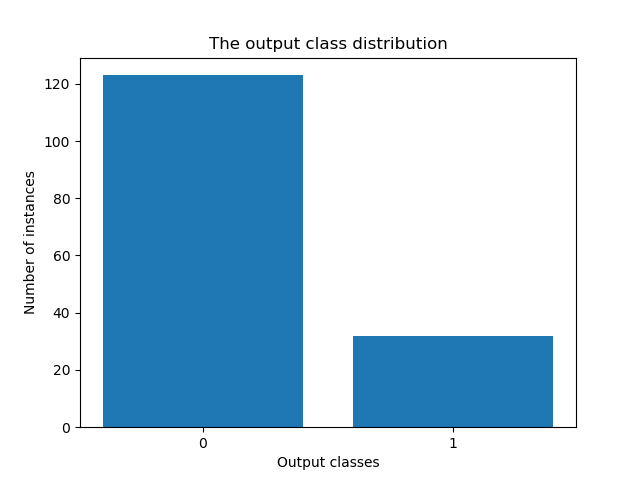
\includegraphics[width=0.8\textwidth]{Hep_Class.png}
				\caption{The class distribution of the output of the hepatitis dataset.}
				\label{fig:HepClass}
			\end{figure}
			
			\item \textit{Numeric feature distributions} (Figure \ref{fig:HepDist}) \\
			These distributions show very clearly how the feature values are distributed and that normalisation and standardisation should be considered to remove the feature value imbalance.
			
			\begin{figure}[H]
				\centering
				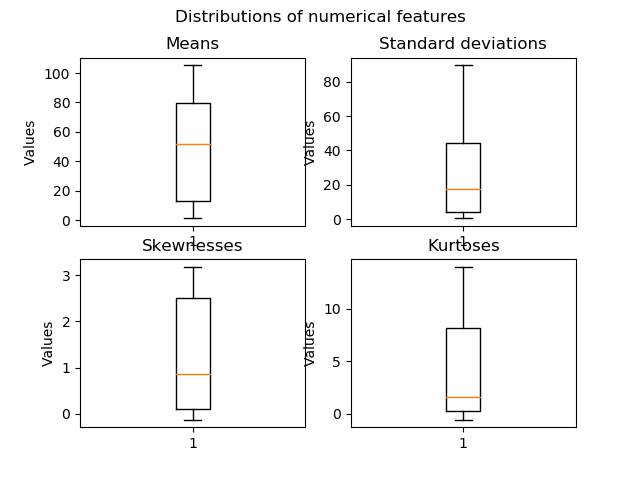
\includegraphics[width=0.8\textwidth]{Hep_Dist.png}
				\caption{The boxplots of the means, standard deviations, skewnesses and kurtoses from the features of the hepatitis dataset.}
				\label{fig:HepDist}
			\end{figure}
			
			\item \textit{Categorical and numeric cardinality} (Figures \ref{fig:HepCardCat} and \ref{fig:HepCardNum}) \\
			The distributions for these cardinality outliers are shown, but not very relevant in this case. No additional information can be found in this case.
			
			\begin{figure}[H]
				\centering
				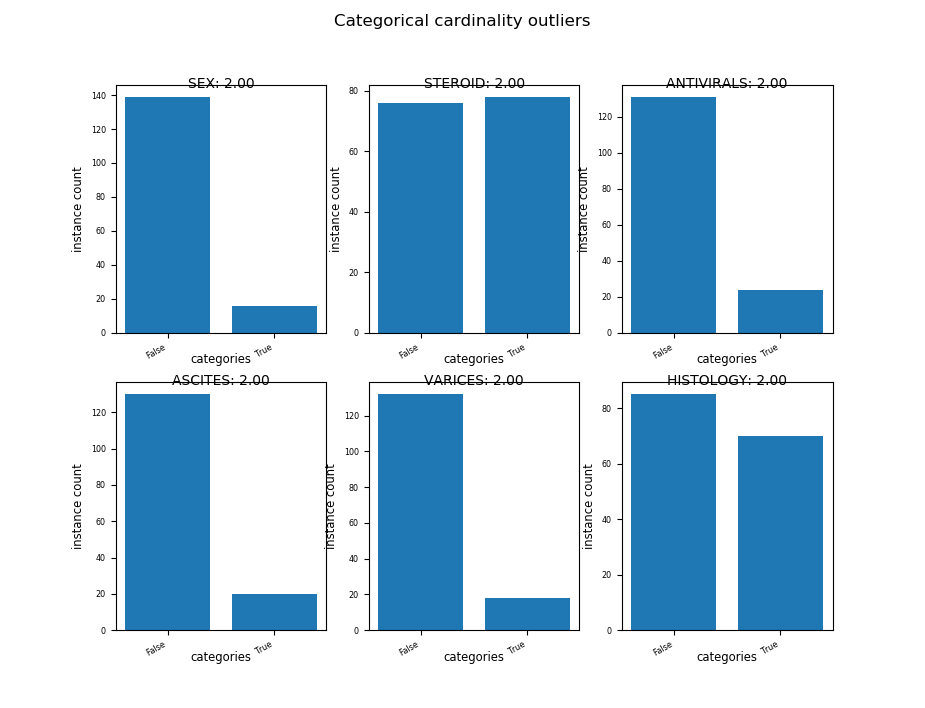
\includegraphics[width=0.8\textwidth]{Hep_Card_Cat.png}
				\caption{Histograms of the categorical features with either the highest or the lowest cardinality in the hepatitis dataset.}
				\label{fig:HepCardCat}
			\end{figure}
			
			\begin{figure}[H]
				\centering
				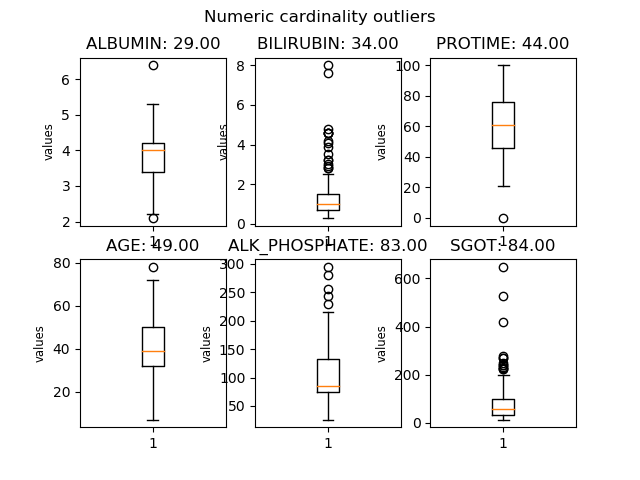
\includegraphics[width=0.8\textwidth]{Hep_Card_Num.png}
				\caption{Boxplots of the numeric features with either the highest or the lowest cardinality in the hepatitis dataset.}
				\label{fig:HepCardNum}
			\end{figure}
			
			\item \textit{Attribute entropy outliers} (Figures \ref{fig:HepAttEntCat} and \ref{fig:HepAttEntNum}) \\
			Especially the figure for categorical distributions show very well how features differ in entropy. The features \textit{SEX}, \textit{VARICES} and \textit{ASCITES} show a strong bias towards the value FALSE.The other three maximum outliers are far more balanced.
			
			\begin{figure}[H]
				\centering
				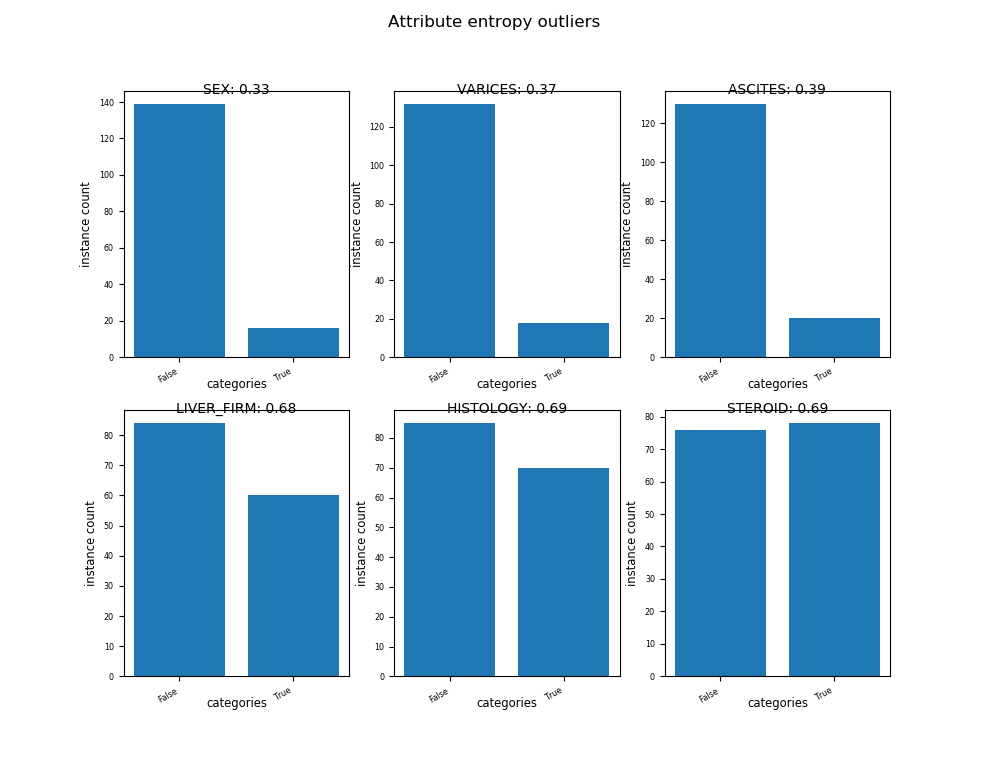
\includegraphics[width=0.8\textwidth]{Hep_AttEnt_Cat.png}
				\caption{Histograms of the categorical features with either the highest or the lowest attribute entropy in the hepatitis dataset.}
				\label{fig:HepAttEntCat}
			\end{figure}
			
			\begin{figure}[H]
				\centering
				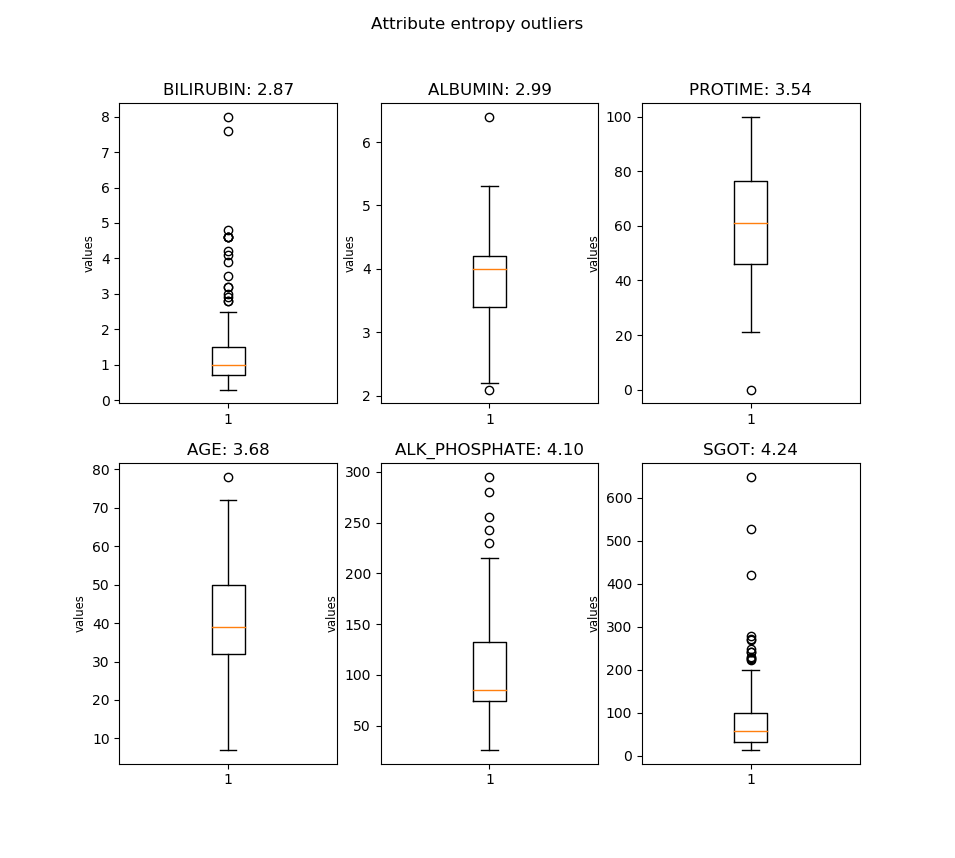
\includegraphics[width=0.8\textwidth]{Hep_AttEnt_Num.png}
				\caption{Boxplots of the numeric features with either the highest or the lowest attribute entropy in the hepatitis dataset.}
				\label{fig:HepAttEntNum}
			\end{figure}
			
		\end{enumerate}
			
	\end{itemize}

	% Final results
	Looking at the overall additional results, several aspects are improved. More insight in correlation is given and several features are known to most likely be irrelevant or to the contrary very relevant. Also the understanding of the issues is better with the histograms and the boxplots.
	
	% MicroOrganisms
	\subsubsection{Micro-organisms Dataset}
	\label{subsec:AdditionalResultMO}
	
	% Introduction
	The additions are shown and discussed per different theme. Also, some of the additions are not discussed, due to lack of relevance. These can still be read (Appendix \ref{app:AdditionalMO}). First the correlation is discussed, followed by the minimum cardinality. Thirdly the outliers are discussed and lastly the plots.
		
	\begin{itemize}
		\item \textit{Correlation:} \\
		
		Due to the imposed restriction of combinatorial explosion, correlation will not be checked for more than 1000 features, and this dataset has 1300 features.
		
		\item \textit{Minimum cardinality} \\
		\underline{Minimum cardinality feature count:} 218 \\

		A total of 218 features have a cardinality of one and therefore do not contain any information. Aside from this, also the names of the 218 features are returned, but not shown due to its size.
		
		\item \textit{Outliers:} \\
		(Table \ref{tab:MOOutliers})
		
		All outliers are computed and the lowest and highest three outliers are shown (Table \ref{tab:MOOutliers}). Some results need further discussion:
		
		\begin{enumerate}
			\item The 20 possible class probabilities show no extreme outliers. Imbalance is still present, but there is no majority problem.
			\item The feature \textit{V1261} has the most potential information and second to most mutual information and therefore is a feature to keep an eye on.
			\item Again the features with one distinct value are found in the lowest outliers.
			\item The closeness in entropy and mutual information for the top three features, shows that far more features are interesting to look at and that these features would be useful.
		\end{enumerate}
		
		\begin{table}[h]
			\caption{The outliers for the micro-organisms dataset}
			\label{tab:MOOutliers}
			\resizebox{\textwidth}{!}{
				\begin{tabular}{l|lll|lll}
					& \multicolumn{3}{l|}{\textbf{Lower bound}}                                                                                                                                                                                          & \multicolumn{3}{l}{\textbf{Upper bound}}                                                                                                                                                                                              \\ \cline{2-7} 
					\textbf{\begin{tabular}[c]{@{}l@{}}Outlier\\ Type\end{tabular}}                                                 & \textbf{\begin{tabular}[c]{@{}l@{}}First\\ Outlier\\ (name)\end{tabular}} & \textbf{\begin{tabular}[c]{@{}l@{}}Second\\ Outlier\\ (name)\end{tabular}} & \textbf{\begin{tabular}[c]{@{}l@{}}Third\\ Outlier\\ (name)\end{tabular}} & \textbf{\begin{tabular}[c]{@{}l@{}}Third\\ Outlier\\ (name)\end{tabular}}   & \textbf{\begin{tabular}[c]{@{}l@{}}Second\\ Outlier\\ (name)\end{tabular}} & \textbf{\begin{tabular}[c]{@{}l@{}}First\\ Outlier\\ (name)\end{tabular}}  \\ \hline
					\multicolumn{1}{|l|}{\textbf{\begin{tabular}[c]{@{}l@{}}Ratio of instances\\ with missing values\end{tabular}}} & \multicolumn{1}{l|}{--}                                                   & \multicolumn{1}{l|}{--}                                                    & --                                                                        & \multicolumn{1}{l|}{--}                                                     & \multicolumn{1}{l|}{--}                                                    & \multicolumn{1}{l|}{--}                                                    \\ \hline
					\multicolumn{1}{|l|}{\textbf{\begin{tabular}[c]{@{}l@{}}Ratio of features\\ with missing values\end{tabular}}}  & \multicolumn{1}{l|}{--}                                                   & \multicolumn{1}{l|}{--}                                                    & --                                                                        & \multicolumn{1}{l|}{--}                                                     & \multicolumn{1}{l|}{--}                                                    & \multicolumn{1}{l|}{--}                                                    \\ \hline
					\multicolumn{1}{|l|}{\textbf{Class probabilities}}                                                              & \multicolumn{1}{l|}{\begin{tabular}[c]{@{}l@{}}0.02\\ (7)\end{tabular}}   & \multicolumn{1}{l|}{\begin{tabular}[c]{@{}l@{}}0.02\\ (6)\end{tabular}}    & \begin{tabular}[c]{@{}l@{}}0.03\\ (9)\end{tabular}                        & \multicolumn{1}{l|}{\begin{tabular}[c]{@{}l@{}}0.09\\ (19)\end{tabular}}    & \multicolumn{1}{l|}{\begin{tabular}[c]{@{}l@{}}0.09\\ (3)\end{tabular}}    & \multicolumn{1}{l|}{\begin{tabular}[c]{@{}l@{}}0.11\\ (11)\end{tabular}}   \\ \hline
					\multicolumn{1}{|l|}{\textbf{\begin{tabular}[c]{@{}l@{}}Categorical\\ cardinality\end{tabular}}}                & \multicolumn{1}{l|}{--}                                                   & \multicolumn{1}{l|}{--}                                                    & --                                                                        & \multicolumn{1}{l|}{--}                                                     & \multicolumn{1}{l|}{--}                                                    & \multicolumn{1}{l|}{--}                                                    \\ \hline
					\multicolumn{1}{|l|}{\textbf{\begin{tabular}[c]{@{}l@{}}Numeric\\ cardinality\end{tabular}}}                    & \multicolumn{1}{l|}{\begin{tabular}[c]{@{}l@{}}1\\ (V1)\end{tabular}}     & \multicolumn{1}{l|}{\begin{tabular}[c]{@{}l@{}}1\\ (V447)\end{tabular}}    & \begin{tabular}[c]{@{}l@{}}1\\ (V1090)\end{tabular}                       & \multicolumn{1}{l|}{\begin{tabular}[c]{@{}l@{}}259\\ (V1261)\end{tabular}}   & \multicolumn{1}{l|}{\begin{tabular}[c]{@{}l@{}}294\\ (V719)\end{tabular}}  & \multicolumn{1}{l|}{\begin{tabular}[c]{@{}l@{}}296\\ (V838)\end{tabular}}  \\ \hline
					\multicolumn{1}{|l|}{\textbf{\begin{tabular}[c]{@{}l@{}}Correlation\\ combinations\end{tabular}}}               & \multicolumn{1}{l|}{--}                                                   & \multicolumn{1}{l|}{--}                                                    & --                                                                        & \multicolumn{1}{l|}{--}                                                     & \multicolumn{1}{l|}{--}                                                    & \multicolumn{1}{l|}{--}                                                    \\ \hline
					\multicolumn{1}{|l|}{\textbf{\begin{tabular}[c]{@{}l@{}}Categorical\\ attribute entropy\end{tabular}}}          & \multicolumn{1}{l|}{--}                                                   & \multicolumn{1}{l|}{--}                                                    & --                                                                        & \multicolumn{1}{l|}{--}                                                     & \multicolumn{1}{l|}{--}                                                    & \multicolumn{1}{l|}{--}                                                    \\ \hline
					\multicolumn{1}{|l|}{\textbf{\begin{tabular}[c]{@{}l@{}}Numeric\\ attribute entropy\end{tabular}}}              & \multicolumn{1}{l|}{\begin{tabular}[c]{@{}l@{}}0.0\\ (V1)\end{tabular}}   & \multicolumn{1}{l|}{\begin{tabular}[c]{@{}l@{}}0.0\\ (V1099)\end{tabular}}  & \begin{tabular}[c]{@{}l@{}}0.0\\ (V212)\end{tabular}                      & \multicolumn{1}{l|}{\begin{tabular}[c]{@{}l@{}}0.60\\ (V1163)\end{tabular}} & \multicolumn{1}{l|}{\begin{tabular}[c]{@{}l@{}}0.62\\ (V1002)\end{tabular}} & \multicolumn{1}{l|}{\begin{tabular}[c]{@{}l@{}}0.83\\ (V1261)\end{tabular}} \\ \hline
					\multicolumn{1}{|l|}{\textbf{\begin{tabular}[c]{@{}l@{}}Categorical\\ joint entropy\end{tabular}}}              & \multicolumn{1}{l|}{--}                                                   & \multicolumn{1}{l|}{--}                                                    & --                                                                        & \multicolumn{1}{l|}{--}                                                     & \multicolumn{1}{l|}{--}                                                    & \multicolumn{1}{l|}{--}                                                    \\ \hline
					\multicolumn{1}{|l|}{\textbf{\begin{tabular}[c]{@{}l@{}}Numeric\\ joint entropy\end{tabular}}}                  & \multicolumn{1}{l|}{\begin{tabular}[c]{@{}l@{}}2.91\\ (V1)\end{tabular}}  & \multicolumn{1}{l|}{\begin{tabular}[c]{@{}l@{}}2.91\\ (V1071)\end{tabular}} & \begin{tabular}[c]{@{}l@{}}2.91\\ (V782)\end{tabular}                     & \multicolumn{1}{l|}{\begin{tabular}[c]{@{}l@{}}3.34\\ (V1163)\end{tabular}} & \multicolumn{1}{l|}{\begin{tabular}[c]{@{}l@{}}3.35\\ (V1002)\end{tabular}} & \multicolumn{1}{l|}{\begin{tabular}[c]{@{}l@{}}3.49\\ (V1261)\end{tabular}} \\ \hline
					\multicolumn{1}{|l|}{\textbf{\begin{tabular}[c]{@{}l@{}}Categorical\\ mutual information\end{tabular}}}         & \multicolumn{1}{l|}{--}                                                   & \multicolumn{1}{l|}{--}                                                    & --                                                                        & \multicolumn{1}{l|}{--}                                                     & \multicolumn{1}{l|}{--}                                                    & \multicolumn{1}{l|}{--}                                                    \\ \hline
					\multicolumn{1}{|l|}{\textbf{\begin{tabular}[c]{@{}l@{}}Numeric\\ mutual information\end{tabular}}}             & \multicolumn{1}{l|}{\begin{tabular}[c]{@{}l@{}}0.00\\ (V1)\end{tabular}}  & \multicolumn{1}{l|}{\begin{tabular}[c]{@{}l@{}}0.00\\ (V251)\end{tabular}} & \begin{tabular}[c]{@{}l@{}}0.00\\ (V248)\end{tabular}                     & \multicolumn{1}{l|}{\begin{tabular}[c]{@{}l@{}}0.25\\ (V787)\end{tabular}} & \multicolumn{1}{l|}{\begin{tabular}[c]{@{}l@{}}0.25\\ (V1261)\end{tabular}} & \multicolumn{1}{l|}{\begin{tabular}[c]{@{}l@{}}0.27\\ (V1008)\end{tabular}} \\ \hline
				\end{tabular}
			}
		\end{table}
		
		\item \textit{Plots} \\
		
		The values for the plots are computed and visualized. Whereas these plots do not show any additional information, they do show earlier mentioned problems:
		
		\underline{Class count histogram:} Figure \ref{fig:MOClass} \\
		
		The class count histogram show that most of the classes are around 25 to 30 instances. There are however seven classes that have significant more or less instances.
		
		\begin{figure}[]
			\centering
			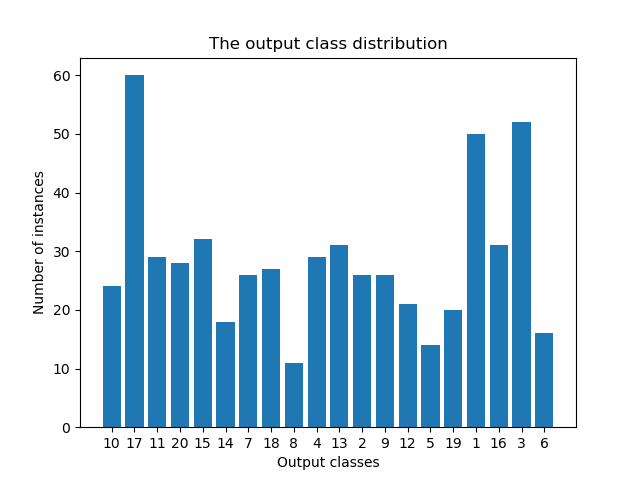
\includegraphics[width=0.8\textwidth]{MO_Class.png}
			\caption{The class distribution of the output of the micro-organisms dataset.}
			\label{fig:MOClass}
		\end{figure}
		
		\underline{Distribution boxplots:} Figure \ref{fig:MODist} \\
		
		These boxplots show very well the difference in values for every feature. The creation of a boxplot of the means and standard deviation and the high number of outliers, show that normalisation or standardisation seems a good preprocessing action.
		
		\begin{figure}[]
			\centering
			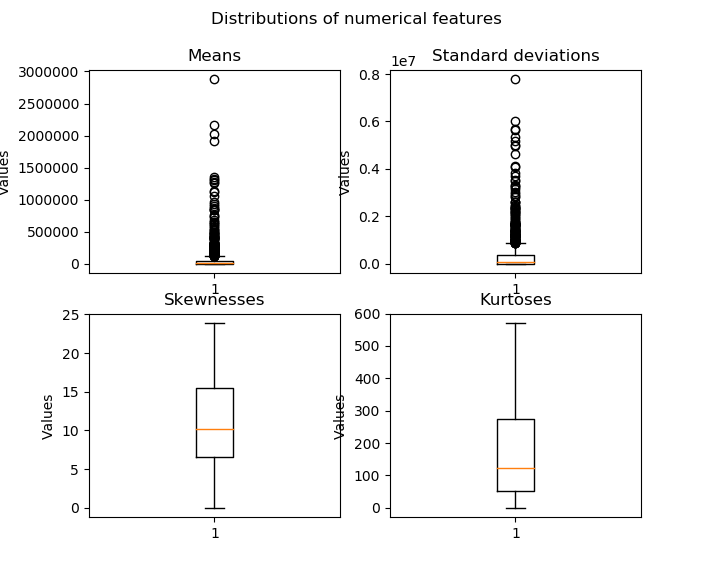
\includegraphics[width=0.8\textwidth]{MO_Dist.png}
			\caption{The boxplots of the means, standard deviations, skewnesses and kurtoses from the features of the micro-organisms dataset.}
			\label{fig:MODist}
		\end{figure}
		
		\underline{Numeric cardinality outlier boxplots:} Figure \ref{fig:MOCardNum} \\
		
		The numeric cardinality boxplots show very well how the feature values are distributed. Due to this dataset orginating from mass spectrometry, most values are 0. All values that are not 0 can become significantly high, with outliers having a factor $10^7$. Again the outliers with the lowest cardinality have just one value, 0.
		
		\begin{figure}[]
			\centering
			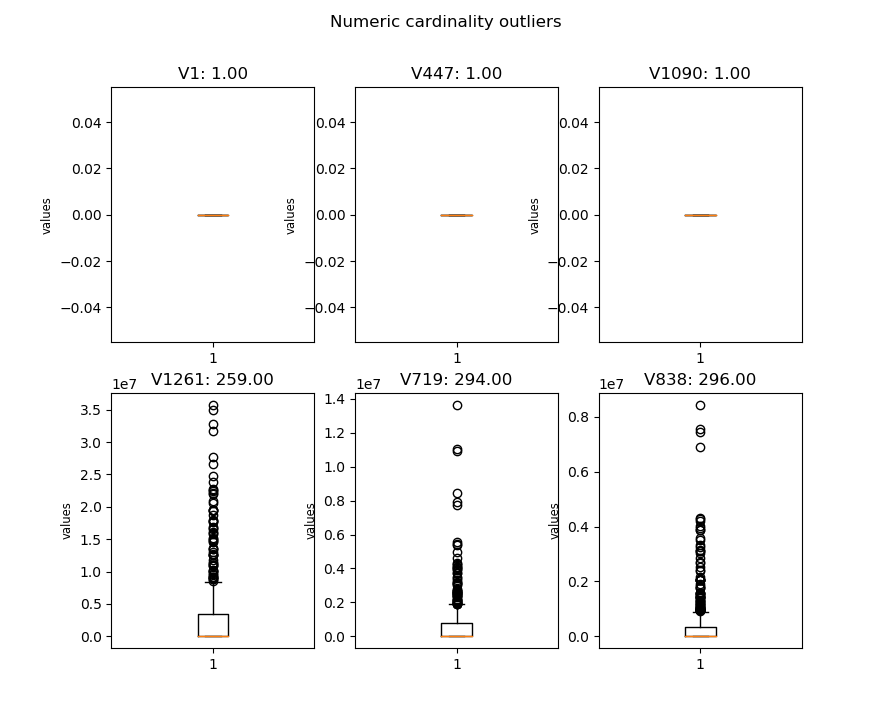
\includegraphics[width=0.8\textwidth]{MO_Card_Num.png}
			\caption{Boxplots of the numeric features with either the highest or the lowest cardinality in the Micro Organisms dataset.}
			\label{fig:MOCardNum}
		\end{figure}
		
		\underline{Numeric attribute entropy boxplots:} Figure \ref{fig:MOAttEntNum} \\
		
		The attribute entropy outliers cannot directly be seen in the box plot. This plot does not seem very useful in this case.
		
		\begin{figure}[]
			\centering
			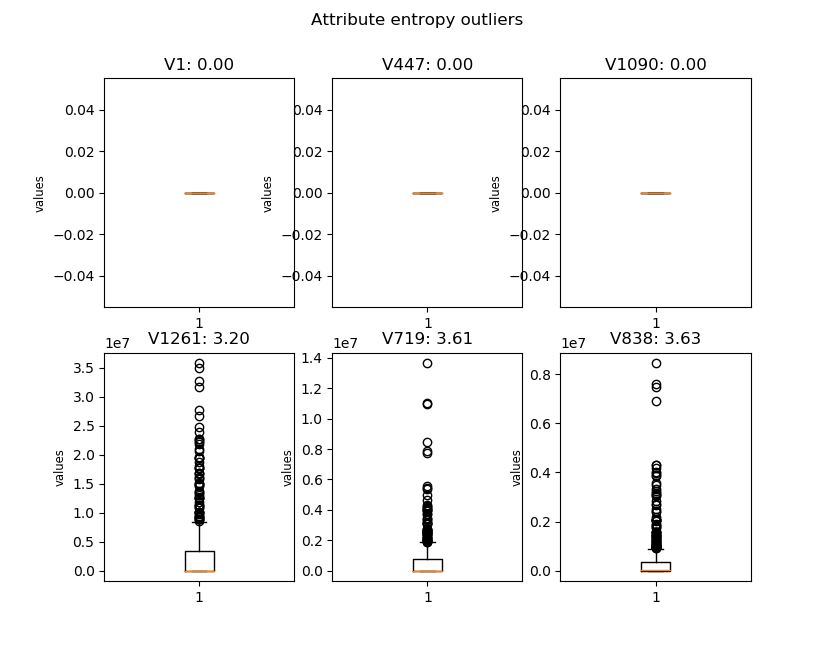
\includegraphics[width=0.8\textwidth]{MO_AttEnt_Num.png}
			\caption{Boxplots of the numeric features with either the highest or the lowest attribute entropy in the Micro organisms dataset.}
			\label{fig:MOAttEntNum}
		\end{figure}
			
	\end{itemize}	
	
	% Final results
	At first finding out that 218 features in the dataset that contain no information is very useful in initial understanding of the dataset. The outliers mainly show that most likely many more features are useful in finding a good result. The histograms and boxplots are more useful as they give a better view in the class distribution. They also visualize the distributions of both the means, standard deviations and also the feature distributions, giving more understanding and insights.
	
	\section{Discussion}
	\label{sec:Discussion}
	
	% Differences in dataset
	There are numerous ways biomedical datasets are gathered and therefore numerous issues that can be found in the dataset. The six discussed issues are well known and therefore a good representation, however there are more issues. For example the issue of having too few instances and trying to generate more is not discussed or the possibility of anomalies being present in the data. These two issues may be addressed in future researches.
	
	% 
		
	\section{Conclusion}
	\label{sec:Conclusions}
	
	% Hypotheses
	The conclusions are based on hypotheses H1 and H2. The first hypothesis H1 is confirmed, in that all issues except for multicollinearity were found in the two datasets with the current meta-features. Multicollinearity would need more addressing besides these meta-features. The information from the meta-features is tough to understand, though. The sheer number of the meta-features makes it hard to find the issues and the lack of examples and visualization makes it hard to how these issues manifest in the dataset, therefore H2 is also confirmed.
	
	% Additions
	The problem posed in the confirmed H2 and the lack of multicollinearity testing in H1 is partly removed by the addition of new meta-features, outliers and histograms and boxplots. These make a better understanding, show several features that need more attention and also show better if multicollinearity can be a problem for the dataset. Therefore the additions are useful for an addition in dataset exploration
	

	
	\bibliography{../References/Citings} 
	\bibliographystyle{ieeetr}
	
	\appendix
	
	\section{Meta-features}
	\label{app:MetaFeatures}
	
	% Introduction
	Meta-features are values gathered out of the dataset. These values can be computed easily with counting aspects or can be found by doing a more extensive analysis. These meta-features show valuable information that can be used for better insights in the dataset and can be used further on in analyses.
	
	\subsection{Basic Meta-features}
	\label{subsec:BasicMF}
	
	% Introduction
	% Metafeature exploration
	The available dataset at the start of a project can have several different important aspects that need to be taken into account. Examples are the size of the dataset and the distribution of the values in it. These dataset aspects are called meta-features\cite{kluegl2009meta}. These meta-features are used in multiple analysis techniques and are an important aspect in meta-learning\cite{kluegl2009meta, castiello2005meta, vilalta2002perspective, bourbakis2011extracting}. These meta-features are also usable without meta-learning however, as they can help by a global exploration of the data. With this exploration directions for preprocessing and analysis can be found, aiding the data analyst in his research. Five different basic meta-feature types are discussed:
	
	% List basic meta-features
	\begin{itemize}
		\item \textbf{Data size} \\
		Finding out the size of the data shows very quickly whether possible limitations or challenges are present. The data size is split into the number of features and the number of samples.
		\item \textbf{Feature types} \\
		There are two main types of features that can be used in a dataset, categorical features and numeric features. Further sub-categorization of the feature types is possible, but is harder to detect. An example of this would be ordinal. Ordinal is categorical data with an order in the categories. In practice, ordinal features either have categorical values with given ordering or numeric values losing the names and are treated as the type they are given.
		\item \textbf{Missing values} \\
		Missing values may be present in the dataset and need some type of processing. This processing can be done in multiple ways which depend on the ratio of missing values as well as the distribution of them over features and samples.
		\item \textbf{Output type} \\
		The output of the dataset can be both categorical and numeric. The type of output changes the choice between using classification and regression respectively. For categorical data, the distribution of the separate categorical classes and whether there are majority and minority classes.
		\item \textbf{Feature cardinalities} \\
		Cardinalities shows the number of unique options available, as there is a significant difference between features with only 2 and with as much as 100 different categories. The same holds for numeric data as with low cardinality the data may be less spread out.
	\end{itemize}
	
	\subsection{Statistical Meta-features}
	\label{subsec:StatisticalMF}
	
	% Introduction
	The dataset can also be approached in a statistical manner. The feature values usually follow a certain distribution. Also similarities between features are worth being looked into. Three statistical meta-feature types are discussed:
	
	% List statistical meta-features
	\begin{itemize}
		\item \textbf{Feature distributions} \\
		The distribution of numeric features is usually shown by using four values, the mean, standard deviation, skewness and kurtosis. The combination of these four indicate distributions that afterwards can be compared for finding difference between distributions
		\item \textbf{Principal component analysis} \\
		An effective way of reducing the number of features by changing them is principal component analysis (PCA). PCA collects the data of all possibly correlated features and creates new uncorrelated features called principal components. To reduce the number of features as much as possible, these principal components are created one by one, giving as much variability to a new principal component as much as possible. Therefore the ratio of total explained variability of the first few principal components can show the presence of correlation within the features and whether feature reduction can be done to lower the dimensionality. In research for which no direct link is needed between input and output, PCA is used to significantly reduce the number of features\cite{wold1987principal}.
		\item \textbf{Correlation} \\
		Whereas PCA creates new uncorrelated features to test variability between them, also a direct look at the correlation can be done by comparing all features with each other\cite{yu2003feature} (Equation \ref{eq:Correlation}). For a high number of features, this can be computationally very exhaustive, however it is a fairly easy way to spot multicollinearity in a dataset\cite{hall2000correlation}.
		
		\begin{equation}\label{eq:Correlation}
		r(x,y) = \frac{\sum_{i}(x_i - \bar{x}_i)(y_i -\bar{y}_i)}{\sum_{i}(x_i - \bar{x}_i)\sum_{i}(y_i -\bar{y}_i)}
		\end{equation}
		
	\end{itemize}
	
	\subsection{Information-theoretic Meta-features}
	\label{subsec:InformationTheoreticMF}
	
	% Introduction
	Information-theoretic meta-features are focused on the information present in the dataset, how useful this information is and if this information is relevant when linking it to the output. These meta-features are focused on the entropy and mutual information and on the combination of these:
	
	% List statistical meta-features
	\begin{itemize}
		\item \textbf{Entropy} \\
		The entropy shows the potential information present in features and the output. Using entropy best works with categorical features, however binning numeric features sometimes can show information gain, too. This information can be seen in the distribution of values over separate categories in categorical data and if the values are more spread out over the categories, the potential information in the feature is higher. This entropy is called attribute entropy is computed by using spreading ratios $r_c$ for every category $c$ (Equation \ref{eq:Entropy}). This spreading ratio $r_c$ is the ratio $r$ of instances that are category $c$.
		
		\begin{equation}\label{eq:Entropy}
		\text{entropy} = - \sum_{c} r_c \log{r_c}
		\end{equation}
		
		The higher the entropy, the more potential information is present. The use of the potential information gain can computed by combining the feature categories and the output classes into new categories and then compute the entropy. If the new so-called joint entropy is very close to the attribute entropy, the potential information can be used to predict output classes and therefore the feature is a good predictor for the output\cite{agresti2003categorical}.
		
		\item \textbf{Mutual information} \\
		Mutual information is another way of matching features with the results. The relevance of using a feature to predict the output is used in the equation to compute mutual information (Equation \ref{eq:MutualInformation})\cite{chow1968approximating}. 
		
		\begin{equation}\label{eq:MutualInformation}
		MI(x, y) = \sum_x \sum_y p(x, y) \log{\frac{p(x, y)}{p(x)p(y)}} dxdy
		\end{equation}
		
		In this equation the probability density function $p$ is used to find the mutual information $MI$ between variables $x$ and $y$\cite{peng2005feature}. A higher mutual information means the feature has a higher predictive power for the output. This mutual information can also be seen as an intersection between the attribute and class entropies.
		
		\item \textbf{Entropy and mutual information} \\
		The outcome values of entropy and mutual information can be combined for measuring ratios between signal and noise. One way to do that is by dividing the class entropy by the averaged mutual information (Equation \ref{eq:EqNumFeat}). The class entropy needs a multitude of features with a certain mutual information for perfect prediction. Since mutual information is lower than the class entropy an estimation can be done for the number of features needed to explain the complete class entropy.
		
		\begin{equation}\label{eq:EqNumFeat}
		\text{equivalent number features} = \frac{\text{class entropy}}{\frac{1}{n}\sum_1^m\text{MI(x)}}
		\end{equation}
		
		A second way of combining attribute entropy and mutual information is by finding out the noise to signal ratio. The attribute entropy of a feature is only partly interesting as not all entropy can be used to predict the output. Mutual information is the part of entropy that can be used in prediction. To find out how much the ratio between noise and information is present, these two can be combined (Equation \ref{eq:NoiseToSignal}).
		
		\begin{equation}\label{eq:NoiseToSignal}
		\text{noise to signal ratio} = \frac{\text{attribute entropy} - \text{MI}}{\text{MI}}
		\end{equation}
		
	\end{itemize}
	
	\subsection{Landmarking Meta-features}
	\label{subsec:LandmarkingMF}
	
	% Introduction
	The quality of analysis can also be tested by performing small analyses. These small analyses can show how well it would perform on the dataset and some small conclusions can be made on them. This is called landmarking, creating very preliminary results in order to reach an outcome\cite{pfahringer2000meta}.
	
	% List landmarking algorithms
	Useful landmarks are based around well known machine learning algorithms. Decision trees are an example of such an algorithm, as it is a well known and easy to understand approach in machine learning.  Other examples are naive bayes, k-nearest neighbour, linear discriminant analysis and logistic regression. Quick analyses can show results that can be used as outcome.
	% Naive bayes, kNN-1, Decision-stump, Random tree degree 1-3, LDA
	
	% List landmarking testees
	These results and therefore the landmarks are based on the quality of the machine learning algorithm. This quality can be measured in multiple ways, such as the accuracy, F1-score and Cohen's kappa.
	
	\section{Meta-feature Values Hepatitis}
	\label{app:MetafeatureValuesHepatitis}
	
	All values for the first analysis for the dataset hepatitis are given here.
	
	\begin{itemize}
		\item \textbf{Basic meta-features}\\
		\begin{enumerate}
			\item \textit{Data size} \\
			\underline{Number of instances:} 155 \\
			\underline{Number of features:} 19\\
			\underline{Number of classes:} 2\\
			\underline{Dimensionality:} 0.12\\
			\item \textit{Data types} \\
			\underline{Number of numeric features:} 6 \\
			\underline{Number of categorical features:} 13 \\
			\underline{Ratio of numeric features:} 0.32 \\
			\underline{Ratio of categorical features:} 0.68 \\
			\item \textit{Missing values} \\
			\underline{Number of missing values:} 167 \\
			\underline{Ratio of missing values:} 0.06 \\
			\underline{Number of instances with missing values:} 75 \\
			\underline{Ratio of instances with missing values:} 0.48 \\
			\underline{Number of features with missing values:} 15 \\
			\underline{Ratio of features with missing values:} 0.79 \\
			\item \textit{Output type} \\
			\underline{Mean of class probability:} 0.5 \\
			\underline{Standard deviation of class probability:} 0.42 \\
			\underline{Minimum of class probability:} 0.21 \\
			\underline{Maximum of class probability:} 0.79 \\
			\underline{Minority class size:} 32 \\
			\underline{Majority class size:} 123 \\					
			\item \textit{Feature cardinalities} \\
			(Table \ref{tab:HepatitisCardinalities})
			\begin{table}[h!]
				\caption{The cardinality meta-features for the Hepatitis dataset}
				\label{tab:HepatitisCardinalities}
				\begin{tabular}{l|l|l}
					\textbf{Cardinality}                                                   & \textbf{\begin{tabular}[c]{@{}l@{}}Categorical\\ features\end{tabular}} & \textbf{\begin{tabular}[c]{@{}l@{}}Numeric\\ features\end{tabular}} \\ \hline
					\textbf{Mean}                                                          & 2                                                                    & 54.67                                                                 \\
					\textbf{\begin{tabular}[c]{@{}l@{}}Standard \\ deviation\end{tabular}} & 0                                                                    & 24.09                                                                 \\ \hline
					\textbf{Minimum}                                                       & 2                                                                       & 30                                                                    \\
					\textbf{Maximum}                                                       & 2                                                                       & 85                                                                   
				\end{tabular}
			\end{table}
		\end{enumerate}
		\item \textbf{Statistical Meta-features} \\
		\begin{enumerate}
			\item \textit{Feature distributions} \\
			(Table \ref{tab:HepatitisFeatureDistributions})
			\begin{table}[h!]
				\caption{The numeric feature distribution of the hepatitis dataset}
				\label{tab:HepatitisFeatureDistributions}
				\begin{tabular}{l|ll|ll}
					\textbf{\begin{tabular}[c]{@{}l@{}}Value \\ distributions\end{tabular}} & \textbf{Means} & \textbf{Standard deviations} & \textbf{Skewnesses} & \textbf{Kurtoses} \\ \hline
					\textbf{Mean}                                                           & 49.92          & 29.74                        & 1.28                & 4.49              \\
					\textbf{\begin{tabular}[c]{@{}l@{}}Standard\\ deviation\end{tabular}}   & 42.57          & 29.73                        & 1.46                & 6.11              \\ \hline
					\textbf{Minimum}                                                        & 1.43           & 0.652                        & -0.12               & -0.53             \\
					\textbf{Maximum}                                                        & 105.33         & 89.65                        & 3.18                & 14.02             \\ \hline
					\textbf{First quartile}                                                 & 13.16          & 89.65                        & 0.11                & 0.25              \\
					\textbf{Second quartile}                                                & 51.53          & 17.72                        & 0.86                & 1.66              \\
					\textbf{Third quartile}                                                 & 79.88          & 44.35                        & 2.51                & 8.18             
				\end{tabular}
			\end{table}  
			\item \textit{Principal component analysis} \\
			\underline{Explained variation component 1:} 0.69 \\
			\underline{Explained variation component 2:} 0.26 \\
			\underline{Explained variation component 3:} 0.04 \\
			\underline{Eigenvalue component 1:} 7919.97 \\
			\underline{Eigenvalue component 2:} 2924.60 \\
			\underline{Eigenvalue component 3:} 412.14 \\
			\underline{Determinant value:} 3.48 \\
		\end{enumerate}
		\item \textbf{Information-theoretic meta-features} \\ 
		\begin{enumerate}
			\item \textit{Entropy} \\
			\underline{Class entropy:} 0.51 \\
			(Table \ref{tab:EntropyMIHepatitisDataset})
			\item \textit{Mutual information} \\
			(Table \ref{tab:EntropyMIHepatitisDataset})
			\begin{table}[h!]
				\caption{The entropies and mutual information values of the hepatitis dataset}
				\label{tab:EntropyMIHepatitisDataset}
				\begin{tabular}{l|llllll}
					\multirow{2}{*}{\textbf{Distributions}} & \multicolumn{3}{l}{\textbf{Categorical features}}                                                                                                                                                                                    & \multicolumn{3}{l}{\textbf{Numeric features}}                                                                                                                                                                   \\ \cline{2-7} 
					& \textbf{\begin{tabular}[c]{@{}l@{}}Attribute\\ entropy\end{tabular}} & \textbf{\begin{tabular}[c]{@{}l@{}}Joint\\ entropy\end{tabular}} & \multicolumn{1}{l|}{\textbf{\begin{tabular}[c]{@{}l@{}}Mutual\\ information\end{tabular}}} & \textbf{\begin{tabular}[c]{@{}l@{}}Attribute\\ entropy\end{tabular}} & \textbf{\begin{tabular}[c]{@{}l@{}}Joint\\ entropy\end{tabular}} & \textbf{\begin{tabular}[c]{@{}l@{}}Mutual\\ information\end{tabular}} \\ \hline
					\textbf{Mean}                           & 0.54                                                                 & 1.01                                                             & \multicolumn{1}{l|}{0.04}                                                                  & 1.02                                                                 & 1.44                                                             & 0.08                                                                  \\
					\textbf{Minimum}                        & 0.33                                                                 & 0.81                                                             & \multicolumn{1}{l|}{0.00}                                                                  & 0.60                                                                 & 1.05                                                             & 0.01                                                                  \\
					\textbf{Maximum}                        & 0.69                                                                 & 1.19                                                             & \multicolumn{1}{l|}{0.09}                                                                  & 1.32                                                                 & 1.80                                                             & 0.17                                                                  \\ \hline
					\textbf{First quartile}                 & 0.43                                                                 & 0.93                                                             & \multicolumn{1}{l|}{0.01}                                                                  & 0.76                                                                 & 1.19                                                             & 0.03                                                                  \\
					\textbf{Second quartile}                & 0.51                                                                 & 1.01                                                             & \multicolumn{1}{l|}{0.03}                                                                  & 1.16                                                                 & 1.50                                                             & 0.6                                                                  \\
					\textbf{Third quartile}                 & 0.67                                                                 & 1.12                                                             & \multicolumn{1}{l|}{0.06}                                                                  & 1.25                                                                 & 1.68                                                             & 0.13                                                                 
				\end{tabular}
			\end{table}
			\item \textit{Entropy and mutual information} \\
			\underline{Equivalent number of categorical features:} 13.8 \\
			\underline{Equivalent number of numeric features:} 6.42 \\
			\underline{Categorical noise to signal ratio:} 13.60 \\
			\underline{Numeric noise to signal ratio:} 11.90 \\
		\end{enumerate}
		\item \textbf{Landmarking meta-features} \\
		(Table \ref{tab:LandmarkingHepatitis})
		
		\begin{table}[h!]
			\caption{The landmarking meta-features of the hepatitis dataset}
			\label{tab:LandmarkingHepatitis}
			\begin{tabular}{l|ll}
				\textbf{\begin{tabular}[c]{@{}l@{}}Machine\\ learning\\ algorithm\end{tabular}}  & \textbf{Error rate} & \textbf{Cohen's kappa} \\ \hline
				\textbf{\begin{tabular}[c]{@{}l@{}}Naive\\ bayes\end{tabular}}                   & 0.22                & 0.48                   \\
				\textbf{\begin{tabular}[c]{@{}l@{}}k-Nearest\\ neighbour\\ (k = 1)\end{tabular}} & 0.32                & 0.15                   \\
				\textbf{\begin{tabular}[c]{@{}l@{}}Decision\\ stump\end{tabular}}                & 0.21                & 0.13                   \\ \hline
				\textbf{\begin{tabular}[c]{@{}l@{}}Random tree\\ (depth = 1)\end{tabular}}       & 0.19                & 0.21                   \\
				\textbf{\begin{tabular}[c]{@{}l@{}}Random tree\\ (depth = 2)\end{tabular}}       & 0.23                & 0.15                   \\
				\textbf{\begin{tabular}[c]{@{}l@{}}Random tree\\ (depth = 3)\end{tabular}}       & 0.27                & 0.21                   \\ \hline
				\textbf{\begin{tabular}[c]{@{}l@{}}Linear\\ Discriminant\end{tabular}}           & 0.17                & 0.46                  
			\end{tabular}
		\end{table}
	\end{itemize}
	
	\section{Meta-feature Values Micro-Organisms}

	\label{app:MetafeatureValuesMO}
	
	All values for the first analysis for the micro organisms are given here.
	
	\begin{itemize}
		\item \textbf{Basic meta-features}\\
		\begin{enumerate}
			\item \textit{Data size} \\
			\underline{Number of instances:} 571 \\
			\underline{Number of features:} 1300 \\
			\underline{Number of classes:} 20 \\
			\underline{Dimensionality:} 2.28\\
			\item \textit{Data types} \\
			\underline{Number of numeric features:} 1300 \\
			\underline{Number of categorical features:} 0 \\
			\underline{Ratio of numeric features:} 1 \\
			\underline{Ratio of categorical features:} 0.0 \\
			\item \textit{Missing values} \\
			\underline{Number of missing values:} 0 \\
			\underline{Ratio of missing values:} 0.0 \\
			\underline{Number of instances with missing values:} 0 \\
			\underline{Ratio of instances with missing values:} 0.0 \\
			\underline{Number of features with missing values:} 0 \\
			\underline{Ratio of features with missing values:} 0.0 \\
			\item \textit{Output type} \\
			\underline{Mean of class probability:} 0.05 \\
			\underline{Standard deviation of class probability:} 0.02 \\
			\underline{Minimum of class probability:} 0.02 \\
			\underline{Maximum of class probability:} 0.1 \\
			\underline{Minority class size:} 11 \\
			\underline{Majority class size:} 60 \\					
			\item \textit{Feature cardinalities} \\
			(Table \ref{tab:MOCardinalities})
			\begin{table}[h!]
				\caption{The cardinality meta-features for the micro organisms dataset}
				\label{tab:MOCardinalities}
				\begin{tabular}{l|l|l}
					\textbf{Cardinality}                                                   & \textbf{\begin{tabular}[c]{@{}l@{}}Categorical\\ features\end{tabular}} & \textbf{\begin{tabular}[c]{@{}l@{}}Numeric\\ features\end{tabular}} \\ \hline
					\textbf{Mean}     &                                                     NaN                                                                    & 45.29                                                                 \\
					\textbf{\begin{tabular}[c]{@{}l@{}}Standard \\ deviation\end{tabular}} & NaN                                                                    & 44.62                                                                 \\ \hline
					\textbf{Minimum}                                                       & NaN                                                                       & 1.0                                                                    \\
					\textbf{Maximum}                                                       & NaN                                                                       & 296                                                                   
				\end{tabular}
			\end{table}
		\end{enumerate}
		\item \textbf{Statistical Meta-features} \\
		\begin{enumerate}
			\item \textit{Feature distributions} \\
			(Table \ref{tab:MOFeatureDistributions})
			\begin{table}[h!]
				\caption{The numeric feature distribution of the micro organisms dataset}
				\label{tab:MOFeatureDistributions}
				\begin{tabular}{l|ll|ll}
					\textbf{\begin{tabular}[c]{@{}l@{}}Value \\ distributions\end{tabular}} & \textbf{Means} & \textbf{Standard deviations} & \textbf{Skewnesses} & \textbf{Kurtoses} \\ \hline
					\textbf{Mean}                                                           & 67437.29          & 343176.13                        & 10.67                & 177.27              \\
					\textbf{\begin{tabular}[c]{@{}l@{}}Standard\\ deviation\end{tabular}}   & 191740.68          & 700237.17                        & 6.95               & 168.76              \\ \hline
					\textbf{Minimum}                                                        & 0.0           & 0.0                        & 0.0               & 0.0             \\
					\textbf{Maximum}                                                        & 2882892.51         & 7792765.65                        & 23.90                & 571.00             \\ \hline
					\textbf{First quartile}                                                 & 696.92          & 9641.40                        & 6.58                & 50.64              \\
					\textbf{Second quartile}                                                & 13117.02          & 94709.23                        & 10.15                & 122.68              \\
					\textbf{Third quartile}                                                 & 50446.57          & 356651.90                        & 15.51                & 274.29             
				\end{tabular}
			\end{table}  
			\item \textit{Principal component analysis} \\
			\underline{Explained variation component 1:} 0.14 \\
			\underline{Explained variation component 2:} 0.10 \\
			\underline{Explained variation component 3:} 0.08 \\
			\underline{Eigenvalue component 1:} 112301000896299.64 \\
			\underline{Eigenvalue component 2:} 83271983089506.69 \\
			\underline{Eigenvalue component 3:} 63192806579339.62 \\
			\underline{Determinant value:} $\infty$ \\
		\end{enumerate}
		\item \textbf{Information-theoretic meta-features} \\ 
		\begin{enumerate}
			\item \textit{Entropy} \\
			\underline{Class entropy:} 2.91 \\
			(Table \ref{tab:EntropyMIMODataset})
			\item \textit{Mutual information} \\
			(Table \ref{tab:EntropyMIMODataset})
			\begin{table}[h!]
				\caption{The entropies and mutual information values of the micro organisms dataset}
				\label{tab:EntropyMIMODataset}
				\begin{tabular}{l|llllll}
					\multirow{2}{*}{\textbf{Distributions}} & \multicolumn{3}{l}{\textbf{Categorical features}}                                                                                                                                                                                    & \multicolumn{3}{l}{\textbf{Numeric features}}                                                                                                                                                                   \\ \cline{2-7} 
					& \textbf{\begin{tabular}[c]{@{}l@{}}Attribute\\ entropy\end{tabular}} & \textbf{\begin{tabular}[c]{@{}l@{}}Joint\\ entropy\end{tabular}} & \multicolumn{1}{l|}{\textbf{\begin{tabular}[c]{@{}l@{}}Mutual\\ information\end{tabular}}} & \textbf{\begin{tabular}[c]{@{}l@{}}Attribute\\ entropy\end{tabular}} & \textbf{\begin{tabular}[c]{@{}l@{}}Joint\\ entropy\end{tabular}} & \textbf{\begin{tabular}[c]{@{}l@{}}Mutual\\ information\end{tabular}} \\ \hline
					\textbf{Mean}                           & NaN                                                                 & NaN                                                             & \multicolumn{1}{l|}{NaN}                                                                  & 0.11                                                                 & 2.98                                                             & 0.04                                                                  \\
					\textbf{Minimum}                        & NaN                                                                 & NaN                                                             & \multicolumn{1}{l|}{NaN}                                                                  & 0.0                                                                 & 2.91                                                             & 0.00                                                                  \\
					\textbf{Maximum}                        & NaN                                                                 & NaN                                                             & \multicolumn{1}{l|}{NaN}                                                                  & 0.83                                                                 & 3.49                                                             & 0.27                                                                  \\ \hline
					\textbf{First quartile}                 & NaN                                                                 & NaN                                                             & \multicolumn{1}{l|}{NaN}                                                                  & 0.03                                                               & 2.93                                                             & 0.01                                                                  \\
					\textbf{Second quartile}                & NaN                                                                 & NaN                                                             & \multicolumn{1}{l|}{NaN}                                                                  & 0.08                                                                 & 2.96                                                             & 0.03                                                                  \\
					\textbf{Third quartile}                 & NaN                                                                 & NaN                                                             & \multicolumn{1}{l|}{NaN}                                                                  & 0.16                                                                 & 3.01                                                             & 0.06                                                                 
				\end{tabular}
			\end{table}
			\item \textit{Entropy and mutual information} \\
			\underline{Equivalent number of categorical features:} NaN \\
			\underline{Equivalent number of numeric features:} 70.27 \\
			\underline{Categorical noise to signal ratio:} NaN \\
			\underline{Numeric noise to signal ratio:} 1.64 \\
		\end{enumerate}
		\item \textbf{Landmarking meta-features} \\
		(Table \ref{tab:LandmarkingMO})
		
		\begin{table}[h!]
			\caption{The landmarking meta-features of the micro organisms dataset}
			\label{tab:LandmarkingMO}
			\begin{tabular}{l|ll}
				\textbf{\begin{tabular}[c]{@{}l@{}}Machine\\ learning\\ algorithm\end{tabular}}  & \textbf{Error rate} & \textbf{Cohen's kappa} \\ \hline
				\textbf{\begin{tabular}[c]{@{}l@{}}Naive\\ bayes\end{tabular}}                   & 0.20                & 0.79                   \\
				\textbf{\begin{tabular}[c]{@{}l@{}}k-Nearest\\ neighbour\\ (k = 1)\end{tabular}} & 0.34                & 0.64                   \\
				\textbf{\begin{tabular}[c]{@{}l@{}}Decision\\ stump\end{tabular}}                & 0.83                & 0.08                   \\ \hline
				\textbf{\begin{tabular}[c]{@{}l@{}}Random tree\\ (depth = 1)\end{tabular}}       & 0.87                & 0.05                   \\
				\textbf{\begin{tabular}[c]{@{}l@{}}Random tree\\ (depth = 2)\end{tabular}}       & 0.78                & 0.14                   \\
				\textbf{\begin{tabular}[c]{@{}l@{}}Random tree\\ (depth = 3)\end{tabular}}       & 0.71                & 0.22                   \\ \hline
				\textbf{\begin{tabular}[c]{@{}l@{}}Linear\\ Discriminant\end{tabular}}           & 0.31                & 0.67                  
			\end{tabular}
		\end{table}
	\end{itemize}
		
\end{document}
